\documentclass[11pt]{article}
\usepackage[utf8]{inputenc}
\usepackage{amsmath,amssymb,amsfonts,amsthm}
\usepackage{graphicx}
\usepackage{xcolor}
\usepackage{hyperref}
\usepackage{geometry}
\usepackage{booktabs}
\usepackage{tcolorbox}
\usepackage{cite}
\geometry{margin=1in}

\newenvironment{acknowledgments}{\section*{Acknowledgments}}{}

% Theorem environments
\newtheorem{theorem}{Theorem}
\newtheorem{lemma}{Lemma}
\newtheorem{proposition}{Proposition}
\newtheorem{corollary}{Corollary}
\newtheorem{definition}{Definition}
\newtheorem{remark}{Remark}
\newtheorem{example}{Example}

\begin{document}

\title{Its From Bits: Mass, Geometry, and Dynamics from\\Gauge-Theoretic Active Inference}

\author{
  Robert C. Dennis\thanks{Corresponding author. Email: cdenn016@gmail.com}\\[0.3cm]
  \small Independent Researcher\\
  \small Leander, Texas, United States\\[0.2cm]
  \small ORCID: \href{https://orcid.org/0009-0004-4688-2341}{0009-0004-4688-2341}
}

\date{\today}

\maketitle

\begin{abstract}
We present a gauge-theoretic active inference framework in which physical quantities---inertial mass, spacetime-like geometry, causal structure, and temporal flow---emerge from multi-agent variational inference on principal $G$-bundles with statistical manifold fibers. Agents are smooth sections of associated bundles carrying beliefs $q_i(c)$, priors $p_i(c)$, and gauge frames $\phi_i(c)$ over a base manifold $\mathcal{C}$, interacting through gauge-covariant transport operators $\Omega_{ij}[\cdot]$ with coupling strengths determined by information-theoretic softmax attention. The central result identifies the Hessian of variational free energy as a natural inertial mass tensor $M = \bar{\Lambda}_p + \Lambda_o + \sum_k \beta_{ik}\tilde{\Lambda}_{q_k} + \sum_j \beta_{ji}\Lambda_{q_i}$, decomposing into prior, sensory, incoming social, and outgoing recoil contributions. Adopting a Hamiltonian ansatz with this mass tensor, we recover Friston's purely dissipative free energy principle as the overdamped limit while predicting oscillation, overshooting, and resonance in underdamped regimes. Computational simulations validate the mass-precision relationship ($R^2 = 0.9998$), energy conservation under symplectic integration, and hierarchical meta-agent emergence across multiple scales. The framework contains standard transformer attention as its zero-dimensional limit, validated through gauge-theoretic transformers achieving $r = 0.821$ correlation with BERT attention patterns and 20\% lower perplexity with 25\% fewer parameters on WikiText-2. Emergent geometry arises via pullback of Fisher-Rao metrics to the base manifold, with critical open problems---particularly the Lorentzian signature problem---clearly identified. This work provides mathematical foundations for Wheeler's participatory universe vision, transitioning ``it from bit'' from philosophy to computational mathematics.
\end{abstract}

\noindent\textbf{Keywords:} Gauge theory $\cdot$ Active inference $\cdot$ Free energy principle $\cdot$ Information geometry $\cdot$ Inertial mass $\cdot$ Emergent spacetime $\cdot$ Transformer architectures

%==============================================================================
\section{Introduction}
\label{sec:intro}
%==============================================================================

\subsection{Wheeler's Vision and the Information-Theoretic Turn}

In 1990, John Archibald Wheeler posed one of the most profound questions in foundations of physics: ``How come existence?'' His answer, encapsulated in the phrase ``it from bit,'' proposed that physical reality derives its existence from information~\cite{Wheeler1990}. Wheeler argued that the universe is fundamentally participatory---the act of observation does not merely reveal pre-existing reality but actively participates in bringing that reality into being: ``no phenomenon is a phenomenon until it is an observed phenomenon''~\cite{Wheeler1983}.

This vision extends beyond quantum mechanics to a cosmological scale. Wheeler proposed a self-referential bootstrap in which observers emerge from physical processes, yet those same observers participate in defining the physical laws and structures from which they arose. Despite its profound implications, Wheeler's vision has remained largely philosophical. While quantum information theory has formalized the ``bit''~\cite{Shannon1948,CoverThomas2006}, and while active inference frameworks have modeled observer behavior~\cite{Friston2010,Friston2017}, no rigorous mathematical framework has united these threads to show how ``it'' can computationally emerge from ``bit.''

Meanwhile, physics has undergone its own conceptual upheavals regarding the nature of spacetime. Jacobson demonstrated that Einstein's field equations can be derived from thermodynamic principles applied to local causal horizons~\cite{Jacobson1995}. Padmanabhan developed complementary thermodynamic formulations~\cite{Padmanabhan2010}. The ER=EPR conjecture~\cite{MaldacenaSusskind2013} and tensor network models~\cite{Swingle2012} suggest that entanglement structure in quantum systems directly encodes geometric relationships. Spacetime, in these frameworks, emerges from patterns of quantum information and correlation.

\subsection{Philosophical Foundation}
\label{sec:philosophy}

Wheeler's participatory universe finds philosophical resonance with Kant's proposal in his 1781 \emph{Critique of Pure Reason}~\cite{Kant1781} that space and time are not properties of things-in-themselves (the \emph{noumena}), but ``forms of sensuous intuition''---constructions of the perceiving mind that organize raw sensory data into coherent experience. Helmholtz advanced this with the brain as an ``unconscious inference'' machine~\cite{Helmholtz1867}, and Friston's Free Energy Principle~\cite{Friston2010} demonstrated that biological systems can be understood as performing approximate Bayesian inference to minimize surprise. We take these insights as motivation: if perception is statistical construction, then the mathematical structures we identify as ``physical'' may themselves be information-theoretic constructions by perceiving agents. We state this philosophical motivation once; the remainder of the paper develops the mathematics.

\subsection{This Work: Contributions and Scope}

We present a mathematical framework for multi-agent interaction that takes cognitive construction seriously. Building on gauge theory, information geometry, and active inference, we model agents as smooth sections of principal bundles carrying beliefs $q_i(c)$, priors $p_i(c)$, and gauge frames $\phi_i(c)$. The framework produces:
\begin{enumerate}
\item A four-component inertial mass tensor arising from the Hessian of variational free energy, identifying mass with statistical precision (Section~\ref{sec:mass})
\item Full Hamiltonian dynamics recovering Friston's gradient flow as the overdamped limit (Section~\ref{sec:dynamics})
\item Computational validation of mass-precision scaling, energy conservation, and hierarchical emergence (Section~\ref{sec:validation})
\item Emergent geometry via pullback of Fisher-Rao metrics to the base manifold (Section~\ref{sec:pullback})
\item Transformer attention as the zero-dimensional limit, validated empirically (Section~\ref{sec:hierarchy})
\end{enumerate}

\subsection{Epistemic Status}
\label{sec:epistemic_status}

This work operates at four distinct epistemic levels, which the reader should keep in mind throughout:

\begin{tcolorbox}[colback=yellow!5,colframe=orange!75,title=Epistemic Distinctions]
\begin{enumerate}
\item \textbf{Mathematical fact:} The identification $M = \partial^2\mathcal{F}/\partial\xi\partial\xi$ as the Hessian of variational free energy is a mathematical result about Fisher information geometry. The four-component mass formula (Eq.~\ref{eq:mass_diagonal}) follows from direct computation.

\item \textbf{Ansatz:} Interpreting this Hessian as inertial mass in a Hamiltonian $\mathcal{H} = \frac{1}{2}\pi^T M^{-1}\pi + \mathcal{F}$ is an \emph{ansatz} motivated by geometric structure, not a derivation from first principles.

\item \textbf{Ansatz-independent predictions:} Overdamped predictions (gradient flow, recovery of classical sociological models) are \emph{independent} of the Hamiltonian ansatz---they require only natural gradient descent on statistical manifolds.

\item \textbf{Ansatz-dependent predictions:} Underdamped predictions (oscillation, resonance, proper time dilation) \emph{depend on the ansatz} and require empirical validation.
\end{enumerate}
\end{tcolorbox}

\textbf{Validated results.} Transformer attention mechanisms emerge as the zero-dimensional limit of gauge-theoretic variational inference. Gauge-theoretic transformers achieve $r = 0.821$ correlation with BERT attention patterns, 20\% lower perplexity on WikiText-2 with 25\% fewer parameters (Section~\ref{sec:hierarchy}). This constitutes falsifiable, empirically confirmed prediction.

\textbf{Mathematical implementation.} Multi-scale participatory dynamics run in working code for systems of 200 agents across 25 hierarchical scales, demonstrating bidirectional information flow (Section~\ref{sec:validation}).

\textbf{Speculative physical interpretation.} Emergent geometry through pullback construction produces Riemannian metrics. Critical problems remain: physical spacetime requires Lorentzian signature (ours is Riemannian), dimensional analysis is incomplete, and quantum connections remain analogical (Sections~\ref{sec:pullback}--\ref{sec:discussion}).

\subsection{Related Work}

Several research programs explore connections between information and spacetime geometry. Jacobson~\cite{Jacobson1995} derived Einstein's field equations from thermodynamic principles; our framework shares information-theoretic foundations but emphasizes multi-agent coordination. Verlinde~\cite{Verlinde2011} proposed gravity from entropic forces; both approaches derive geometry from information, but through different mechanisms. Swingle~\cite{Swingle2012} showed tensor networks model AdS/CFT correspondence; our framework uses classical information geometry rather than quantum entanglement. Constructor theory~\cite{Deutsch2015} and quantum information approaches~\cite{Cao2017} explore geometry from quantum structures; our framework implements through gauge theory with classical distributions. Our approach uniquely combines explicit gauge structure, hierarchical multi-scale organization, computational implementation, and empirical validation through transformer emergence.

\subsection{Notation}
\label{sec:notation}

Table~\ref{tab:notation} summarizes key notation used throughout this paper.

\begin{table}[h]
\centering
\small
\begin{tabular}{ll}
\toprule
\textbf{Symbol} & \textbf{Meaning} \\
\midrule
$\mathcal{C}$ & Base (noumenal) manifold \\
$\mathcal{B}_q, \mathcal{B}_p$ & Statistical manifolds of beliefs and priors \\
$q_i(c) = \mathcal{N}(\mu_i, \Sigma_i)$ & Agent $i$'s belief distribution at $c$ \\
$p_i(c) = \mathcal{N}(\bar{\mu}_i, \bar{\Sigma}_i)$ & Agent $i$'s prior distribution at $c$ \\
$\phi_i(c) \in \mathfrak{g}$ & Agent $i$'s gauge frame field \\
$G = \mathrm{SO}(N)$ & Structure group (gauge group) \\
$\Omega_{ij}[\cdot]$ & Gauge transport operator: $\Omega_{ij} = e^{\phi_i}e^{-\phi_j}$ \\
$\Lambda_{q_i} = \Sigma_i^{-1}$ & Belief precision \\
$\bar{\Lambda}_{p_i} = \bar{\Sigma}_i^{-1}$ & Prior precision \\
$\Lambda_{o_i} = \Sigma_{o_i}^{-1}$ & Observation precision \\
$\tilde{\Lambda}_{q_k} = \Omega_{ik}\Lambda_{q_k}\Omega_{ik}^T$ & Transported precision \\
$\beta_{ij}(c)$ & Belief attention weight (softmax over KL) \\
$\gamma_{ij}(c)$ & Model attention weight \\
$\mathcal{F}$ & Variational free energy functional \\
$M$ & Mass matrix (Hessian of $\mathcal{F}$) \\
$g_{\mathcal{B}}$ & Fisher-Rao metric on statistical manifold \\
\bottomrule
\end{tabular}
\caption{Key notation. Transport operators use bracket notation $\Omega_{ij}[\cdot]$ consistently throughout.}
\label{tab:notation}
\end{table}

%==============================================================================
\section{Gauge-Theoretic Framework}
\label{sec:framework}
%==============================================================================

\subsection{The Core Idea}

The framework rests on a simple but powerful idea: agents are smooth probability distributions evolving over an abstract space, coupled through information exchange, with each agent viewing reality through its own internal reference frame. We formalize this through three mathematical ingredients: a base manifold $\mathcal{C}$ representing the underlying reality about which agents form beliefs, statistical manifolds of probability distributions equipped with information-geometric structure, and gauge theory on principal bundles enabling agents to maintain distinct perspectives while comparing beliefs through transport operators.

\subsection{Base Manifold}

\begin{definition}[Base Manifold]
The base space $\mathcal{C}$ is a smooth $n$-dimensional manifold representing the noumenal substrate over which agents maintain probability distributions.
\end{definition}

$\mathcal{C}$ is \emph{not} physical spacetime. Physical space and time will emerge as induced structures when agents pull back metrics from their belief fields (Section~\ref{sec:pullback}). The base manifold is logically prior to spacetime. We use local coordinates $c = (c^1, \ldots, c^n)$ on $\mathcal{C}$.

\subsection{Statistical Manifolds}

\begin{definition}[Statistical Manifolds]
Let $\mathcal{B}_q$ and $\mathcal{B}_p$ denote the manifolds of belief and prior distributions, each equipped with the Fisher-Rao metric:
\begin{equation}
g_{\mathcal{B}}(\partial_i, \partial_j) = \mathbb{E}_{q}\left[(\partial_i \log q)(\partial_j \log q)\right]
\end{equation}
\end{definition}

The Fisher-Rao metric is unique up to scaling as the only Riemannian metric on probability spaces invariant under sufficient statistics~\cite{Cencov1982}. We use Gaussian statistical manifolds $\mathcal{B} = \{\mathcal{N}(\mu, \Sigma) : \mu \in \mathbb{R}^K, \Sigma \succ 0\}$. The KL divergence between Gaussians has closed form:
\begin{equation}
\mathrm{KL}(\mathcal{N}(\mu_1, \Sigma_1) \| \mathcal{N}(\mu_2, \Sigma_2)) = \frac{1}{2}\left[\log\frac{|\Sigma_2|}{|\Sigma_1|} + \mathrm{tr}(\Sigma_2^{-1}\Sigma_1) + (\mu_2 - \mu_1)^\top\Sigma_2^{-1}(\mu_2 - \mu_1) - K\right]
\label{eq:kl_gaussian}
\end{equation}

\subsection{Principal Bundles and Gauge Freedom}

Different agents use different internal reference frames. This gauge freedom is encoded in a principal bundle.

\begin{definition}[Principal Bundle]
Let $\pi: \mathcal{N} \to \mathcal{C}$ be a principal $G$-bundle where $\mathcal{N}$ is the total space, $\mathcal{C}$ is the base manifold, and $G$ (typically $\mathrm{SO}(N)$) acts freely on $\mathcal{N}$.
\end{definition}

The associated bundles $\mathcal{E}_q = \mathcal{N} \times_{\rho_q} \mathcal{B}_q$ and $\mathcal{E}_p = \mathcal{N} \times_{\rho_p} \mathcal{B}_p$ attach statistical manifolds to gauge structure. For Gaussians with $G = \mathrm{SO}(N)$, the representation acts by $\rho(g) \cdot \mathcal{N}(\mu, \Sigma) = \mathcal{N}(g\mu, g\Sigma g^\top)$.

\subsection{Agents as Smooth Sections}

\begin{definition}[Agent]
An agent $\mathcal{A}^i$ with support domain $\mathcal{U}_i \subseteq \mathcal{C}$ consists of three smooth fields:
\begin{align}
q_i &: \mathcal{U}_i \to \mathcal{E}_q|_{\mathcal{U}_i}, \quad \text{(belief section)} \\
p_i &: \mathcal{U}_i \to \mathcal{E}_p|_{\mathcal{U}_i}, \quad \text{(prior section)} \\
\phi_i &: \mathcal{U}_i \to \mathfrak{g}, \quad \text{(gauge frame field)}
\end{align}
\end{definition}

For Gaussian agents: $q_i(c) = \mathcal{N}(\mu_i(c), \Sigma_i(c))$, $p_i(c) = \mathcal{N}(\bar{\mu}_i(c), \bar{\Sigma}_i(c))$, and $\phi_i(c) = \phi_i^a(c) G_a$ where $\{G_a\}$ are generators of $\mathfrak{so}(N)$.

\subsection{Transport Operators and Gauge Covariance}

When agents $i$ and $j$ overlap at $c \in \mathcal{U}_i \cap \mathcal{U}_j$, the transport operator is:
\begin{equation}
\Omega_{ij}(c) = \exp[\phi_i(c)] \exp[-\phi_j(c)] \in G
\end{equation}

This operator transforms agent $j$'s representations into agent $i$'s frame. It acts on distributions through $\Omega_{ij}[q_j](c) := \rho(\Omega_{ij}(c))\, q_j(c)$. For Gaussians: $\Omega_{ij}[q_j] = \mathcal{N}(\Omega_{ij}\mu_j, \Omega_{ij}\Sigma_j\Omega_{ij}^\top)$.

All meaningful quantities must be invariant under simultaneous gauge transformations $\phi_i(c) \to \phi_i(c) + \xi(c)$ for all $i$. The transport operator satisfies this: $\Omega_{ij} \to \exp(\phi_i + \xi)\exp(-(\phi_j + \xi)) = \Omega_{ij}$. Only relative frames matter.

The gauge frame induces a connection one-form $A^{(i)}_\mu(c) = U_i^{-1}(c)\partial_\mu U_i(c)$ where $U_i = \exp[\phi_i]$, and field strength $F^{(i)}_{\mu\nu} = \partial_\mu A^{(i)}_\nu - \partial_\nu A^{(i)}_\mu + [A^{(i)}_\mu, A^{(i)}_\nu]$ measuring path-dependence of information transport.

\subsection{Multi-Agent Systems and Epistemic Death}

\begin{definition}[Multi-Agent System]
$\mathcal{M} = \{\mathcal{A}^i = (q_i, p_i, \phi_i)\}_{i \in \mathcal{I}}$ over base manifold $\mathcal{C}$, with overlapping domains $\mathcal{U}_i \cap \mathcal{U}_j \neq \emptyset$.
\end{definition}

\begin{definition}[Epistemic Death]
\label{def:epistemic_death}
A set of agents $\{i, j, \ldots\}$ is epistemically dead if:
\begin{align}
\mathrm{KL}(q_i(c) \| \Omega_{ij}[q_j](c)) &= 0 \\
\mathrm{KL}(p_i(c) \| \Omega_{ij}[p_j](c)) &= 0
\end{align}
for all $c$ and all pairs $(i,j)$, \emph{and} observation terms vanish: $\Lambda_{o_i} = 0$ for all $i$.
\end{definition}

We distinguish two phenomena that are sometimes conflated: \emph{complete informational consensus}, where agents agree on everything after transport, and \emph{cessation of dynamics}, where no free energy gradients remain. Consensus alone does not imply epistemic death---agents could agree on beliefs while still having observation-driven dynamics. Epistemic death requires both consensus \emph{and} vanishing observation terms.

\subsection{Working Simplifications}

For this initial study: matched bundles ($\mathcal{B}_q = \mathcal{B}_p$), Gaussian fibers, $\mathrm{SO}(3)$ gauge group, flat base manifold $\mathcal{C} = \mathbb{R}^2$, and smooth gauge frames with negligible local field strength. These are practical choices preserving gauge covariance, information-geometric dynamics, and multi-scale emergence.

%==============================================================================
\section{Multi-Agent Free Energy}
\label{sec:free_energy}
%==============================================================================

\subsection{The Variational Free Energy Principle}

The variational free energy provides an upper bound on surprise: $F[q] = \mathrm{KL}(q(x) \| p(x \mid o)) - \log p(o) \geq -\log p(o)$ for any approximate posterior $q(x)$~\cite{Friston2010,Parr2022}. Minimizing $F$ simultaneously maximizes evidence and minimizes divergence from the true posterior.

\subsection{Multi-Agent Extension}

We extend to multiple interacting agents by introducing auxiliary ``agreement'' variables $z_{ij}$ mediating belief alignment through a normalized probabilistic model. After integrating out auxiliary variables (see Supplementary Information~\cite{Dennis2025supp} for derivation), the free energy becomes:

\begin{equation}
\boxed{
\begin{aligned}
\mathcal{F}[\{q_i\}, \{p_i\}, \{\phi_i\}]
&= \sum_i \int_{\mathcal{C}} \chi_i(c) \, \mathrm{KL}(q_i(c) \| p_i(c)) \, dc \\
&\quad + \sum_{ij} \int_{\mathcal{C}} \chi_{ij}(c) \, \beta_{ij}(c) \, \mathrm{KL}(q_i(c) \| \Omega_{ij}[q_j(c)]) \, dc \\
&\quad + \sum_{ij} \int_{\mathcal{C}} \chi_{ij}(c) \, \gamma_{ij}(c) \, \mathrm{KL}(p_i(c) \| \Omega_{ij}[p_j(c)]) \, dc \\
&\quad - \sum_i \int_{\mathcal{C}} \chi_i(c) \, \mathbb{E}_{q_i(c)}[\log p(o(c) \mid q_i(c))] \, dc
\end{aligned}
}
\label{eq:free_energy}
\end{equation}

where the attention weights are:
\begin{equation}
\beta_{ij}(c) = \frac{\exp\left[-\tau^{-1}\mathrm{KL}(q_i(c) \| \Omega_{ij}[q_j(c)])\right]}{\sum_k \exp\left[-\tau^{-1}\mathrm{KL}(q_i(c) \| \Omega_{ik}[q_k(c)])\right]}
\label{eq:attention}
\end{equation}
and similarly for $\gamma_{ij}(c)$.

\subsection{Interpretation of Terms}

The \emph{self-consistency} term $\sum_i \mathrm{KL}(q_i \| p_i)$ penalizes beliefs deviating from priors. The \emph{belief alignment} term drives agents toward consensus after gauge transport, with attention $\beta_{ij}(c)$ creating positive feedback: agreement increases attention, which further drives consensus. The \emph{model alignment} term aligns generative models, creating shared ontologies. The \emph{observation likelihood} grounds the system in empirical reality.

The attention field $\beta_{ij}(c)$ is not hand-crafted but emerges from variational free energy minimization (Fig.~\ref{fig:attention}).

\begin{figure}[t]
\centering
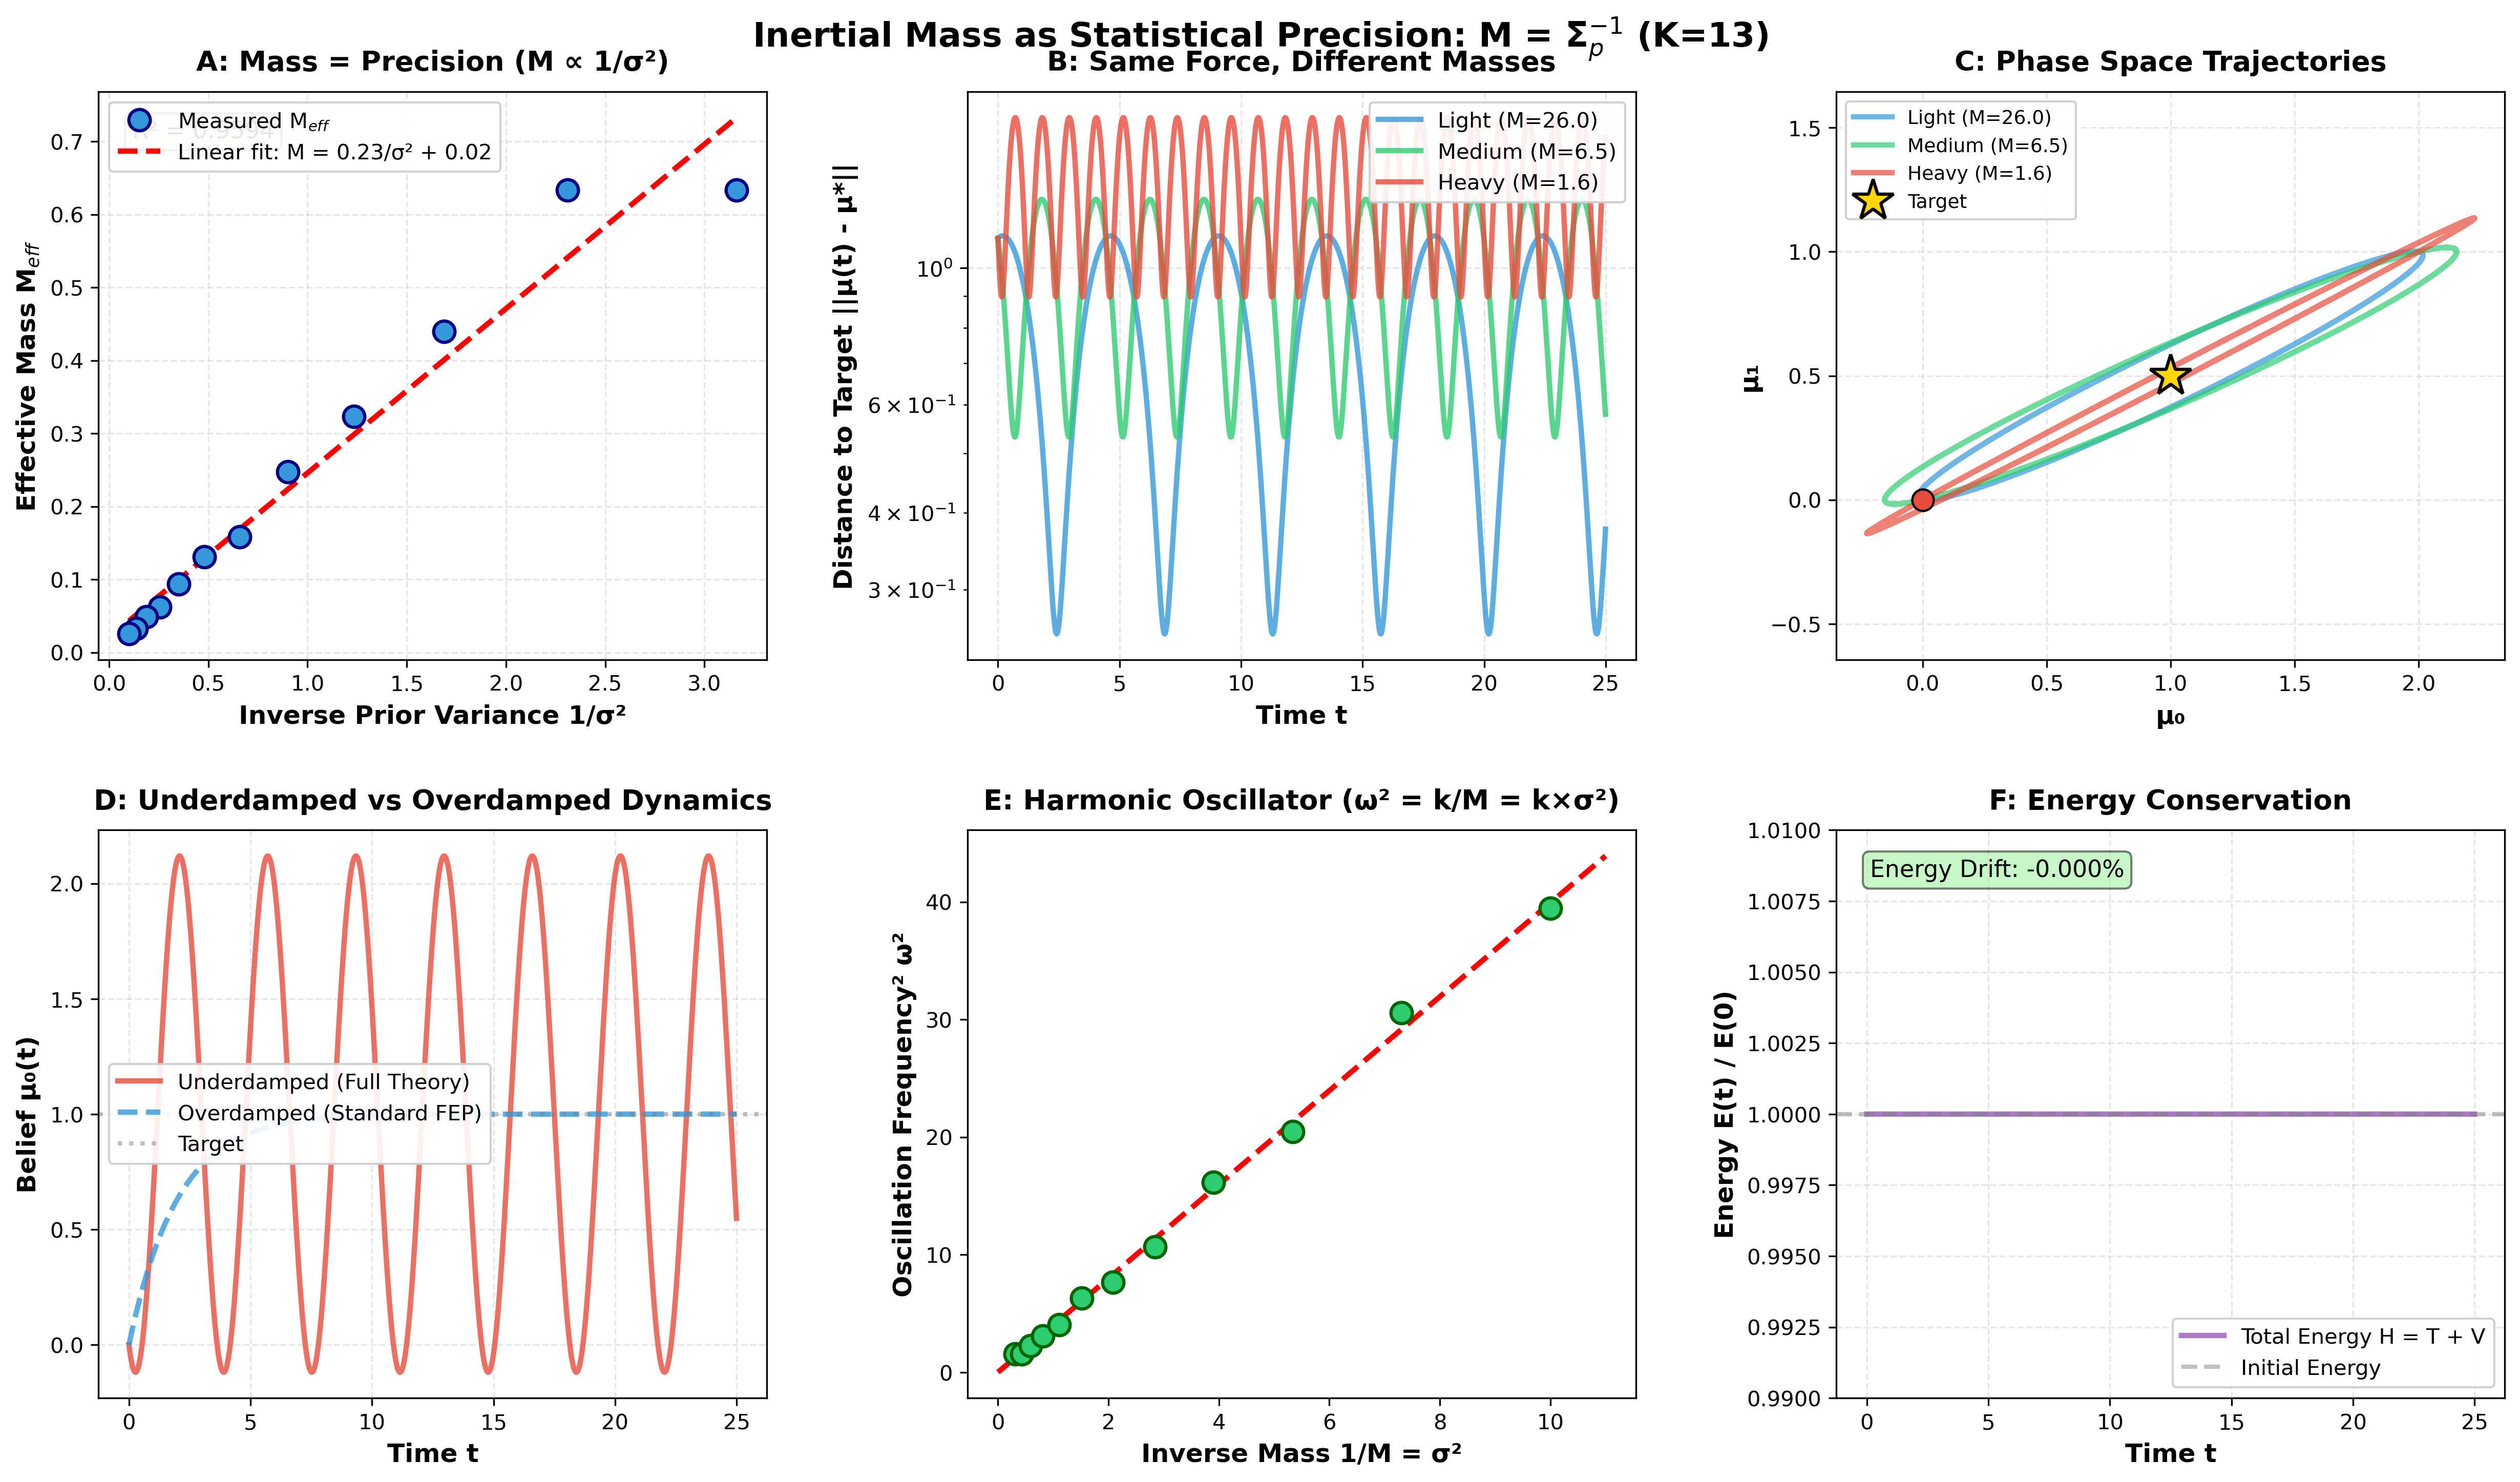
\includegraphics[width=0.55\linewidth]{Fig_1.png}
\caption{Belief attention field $\beta_{ij}(c)$ between two agents across the base manifold. Warm colors indicate high attention (informational alignment); cool colors indicate low attention (divergence). The spatial structure arises from variational free energy minimization, not learned weights.}
\label{fig:attention}
\end{figure}

\subsection{Observations as Agents}

Observation terms can be eliminated by treating environmental stimuli as additional agents with sharp beliefs. For each observation $o_k$, an environmental agent $e_k$ with sharp belief $q_{e_k}$ couples through $\beta_{i,e_k}\mathrm{KL}(q_i \| \Omega_{i,e_k}[q_{e_k}])$, yielding equivalent gradient flows. This produces a fully self-contained framework where everything is an agent.

\subsection{Timescale Hierarchy}

The system exhibits natural timescale separation: fast belief dynamics ($\eta_q \sim \mathcal{O}(1)$), slow model learning ($\eta_p \ll \eta_q$), and very slow gauge frame evolution ($\eta_\phi \sim \eta_p$), with characteristic ratio $\eta_q : \eta_p : \eta_\phi \sim 1 : \epsilon : \epsilon^2$. This enables adiabatic approximation analogous to Born-Oppenheimer in molecular physics~\cite{Born1927}.

\subsection{Spontaneous Symmetry Breaking}

Without observations, agents converge to a gauge-symmetric equilibrium occupying a gauge orbit (Fig.~\ref{fig:symmetry}). When agents receive observations, this symmetry breaks spontaneously: agents flow toward unique states as agents specialize, mirroring Goldstone mode emergence in continuous symmetry breaking.

\begin{figure}[t]
\centering
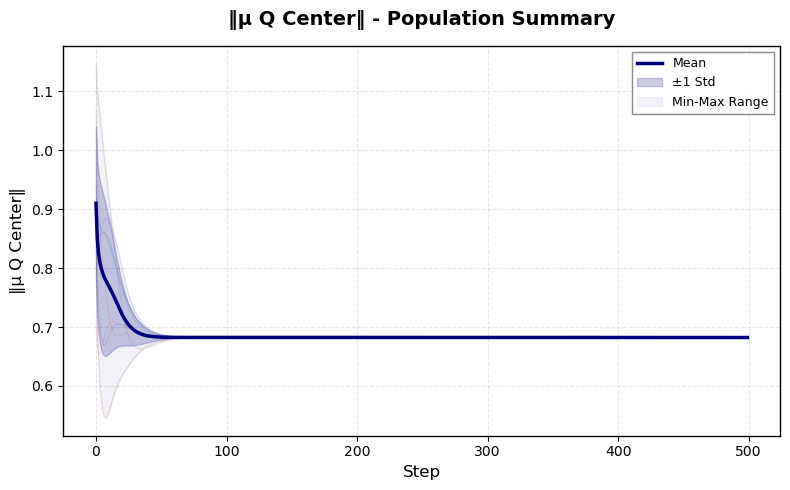
\includegraphics[width=0.48\linewidth]{Fig_2_top.png}
\hfill
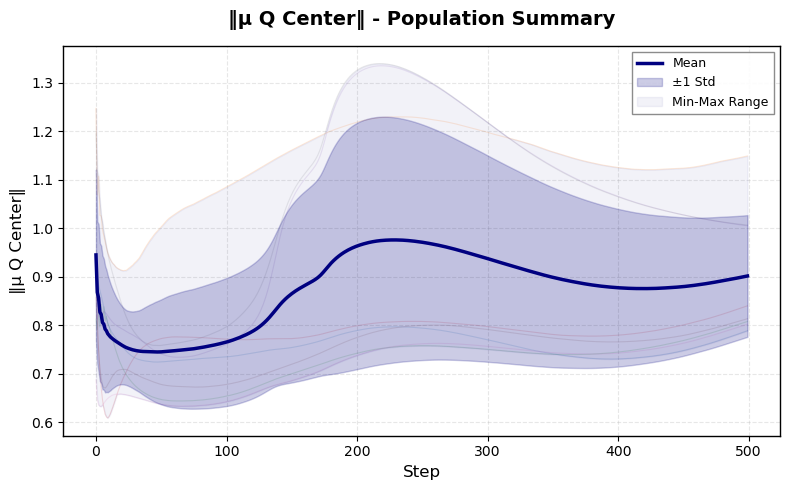
\includegraphics[width=0.48\linewidth]{Fig_3_top.png}
\caption{\textbf{Left:} Vacuum state without observations---all agents converge to identical belief magnitudes, occupying a gauge orbit (unbroken symmetry). \textbf{Right:} Observation-driven symmetry breaking---agents flow toward unique values, demonstrating specialization analogous to Goldstone modes.}
\label{fig:symmetry}
\end{figure}
%==============================================================================
\section{Mass from Statistical Precision}
\label{sec:mass}
%==============================================================================

The variational free energy $\mathcal{F}$ serves as the potential for agent dynamics. We now show that its second-order structure reveals a kinetic energy term identifying inertial mass with statistical precision. We work in the quasi-static approximation where prior parameters $(\bar{\mu}_i, \bar{\Sigma}_i)$ evolve slowly relative to beliefs $(\mu_i, \Sigma_i)$.

\subsection{Setup and Notation}

Each agent $i$ maintains belief $q_i = \mathcal{N}(\mu_i, \Sigma_i)$ anchored to prior $p_i = \mathcal{N}(\bar{\mu}_i, \bar{\Sigma}_i)$ and receives observations $o_i$ through likelihood $p(o_i|\theta) = \mathcal{N}(o_i; \theta, \Sigma_{o_i})$, with precisions $\Lambda_{q_i} = \Sigma_i^{-1}$, $\bar{\Lambda}_{p_i} = \bar{\Sigma}_i^{-1}$, $\Lambda_{o_i} = \Sigma_{o_i}^{-1}$, and transported quantities $\tilde{\mu}_k = \Omega_{ik}\mu_k$, $\tilde{\Lambda}_{q_k} = \Omega_{ik}\Lambda_{q_k}\Omega_{ik}^T$.

\subsection{The Extended Free Energy}

The complete variational free energy with sensory evidence is:
\begin{equation}
\mathcal{F}[\{q_i\}] = \sum_i \mathrm{KL}(q_i \| p_i) + \sum_{i,k}\beta_{ik}\mathrm{KL}(q_i \| \Omega_{ik}[q_k]) - \sum_i \mathbb{E}_{q_i}[\log p(o_i|\theta)]
\label{eq:extended_F}
\end{equation}
representing prior anchoring, social consensus, and sensory evidence.

\subsection{First Variations}

The total gradient with respect to agent $i$'s mean is:
\begin{equation}
\frac{\partial\mathcal{F}}{\partial\mu_i} = \bar{\Lambda}_{p_i}(\mu_i - \bar{\mu}_i) + \sum_k\beta_{ik}\tilde{\Lambda}_{q_k}(\mu_i - \tilde{\mu}_k) + \sum_j\beta_{ji}\Lambda_{q_i}\Omega_{ji}^T(\tilde{\mu}_i^{(j)} - \mu_j) + \Lambda_{o_i}(\mu_i - o_i)
\label{eq:gradient}
\end{equation}
where $\tilde{\mu}_i^{(j)} = \Omega_{ji}\mu_i$ is agent $i$'s mean transported into agent $j$'s frame.

\subsection{Second Variations: The Mass Matrix}

The Hessian $M = \partial^2\mathcal{F}/\partial\xi\partial\xi$ with state vector $\xi = (\mu_1, \ldots, \mu_N, \Sigma_1, \ldots, \Sigma_N)$ has block structure:
\begin{equation}
M = \begin{pmatrix} M_{\mu\mu} & C^{\mu\Sigma} \\ (C^{\mu\Sigma})^T & M_{\Sigma\Sigma} \end{pmatrix}
\end{equation}

\subsubsection{Mean Sector: Diagonal Blocks}

The diagonal mass for agent $i$ receives four contributions---from the prior, consensus as receiver, consensus as sender, and sensory evidence:

\begin{equation}
\boxed{[M_{\mu\mu}]_{ii} = \underbrace{\bar{\Lambda}_{p_i}}_{\text{prior (bare mass)}} + \underbrace{\sum_k \beta_{ik}\tilde{\Lambda}_{q_k}}_{\text{incoming social}} + \underbrace{\sum_j \beta_{ji}\Lambda_{q_i}}_{\text{outgoing recoil}} + \underbrace{\Lambda_{o_i}}_{\text{sensory}}}
\label{eq:mass_diagonal}
\end{equation}

Each component has clear physical interpretation. The \emph{bare mass} $\bar{\Lambda}_{p_i}$ provides inertia against deviation from the prior world-model: an agent with precise priors resists belief change. The \emph{incoming social mass} captures inertia from being pulled by neighbors---the more precise the neighbors' transported beliefs, the heavier the agent. The \emph{outgoing recoil mass} represents inertia from pulling neighbors (Newton's third law analog). The \emph{sensory mass} grounds the agent in observations.

\subsubsection{Mean Sector: Off-Diagonal Blocks}

\begin{equation}
\boxed{[M_{\mu\mu}]_{ik} = -\beta_{ik}\Omega_{ik}\Lambda_{q_k} - \beta_{ki}\Lambda_{q_i}\Omega_{ki}^T \quad (i \neq k)}
\label{eq:mass_offdiag}
\end{equation}

The mass matrix is symmetric only when $\beta_{ik} = \beta_{ki}$ and $\Omega_{ik} = \Omega_{ki}^T$.

\subsubsection{Covariance Sector}

Diagonal blocks:
\begin{equation}
[M_{\Sigma\Sigma}]_{ii} = \frac{1}{2}(\Lambda_{q_i} \otimes \Lambda_{q_i})\left(1 + \sum_k\beta_{ik} + \sum_j\beta_{ji}\right)
\label{eq:mass_cov}
\end{equation}

The sensory precision $\Lambda_{o_i}$ contributes to mean-sector mass but not covariance-sector mass.

\subsubsection{Cross Blocks}

$[C^{\mu\Sigma}]_{ik} = 0$ when $\mu_i = \tilde{\mu}_k$ (at consensus), so the mean and covariance sectors decouple near equilibrium.

\subsection{Stability of the Coupled Mass Matrix}
\label{sec:stability}

For well-posed Hamiltonian dynamics, $M_{\mu\mu}$ must be positive-definite. We establish conditions under which this holds.

\begin{proposition}[Positive-Definiteness via Diagonal Dominance]
If for each agent $i$:
\begin{equation}
\bar{\Lambda}_{p_i} + \Lambda_{o_i} + \sum_k\beta_{ik}\tilde{\Lambda}_{q_k} + \sum_j\beta_{ji}\Lambda_{q_i} > \sum_{k \neq i}\left|\beta_{ik}\Omega_{ik}\Lambda_{q_k} + \beta_{ki}\Lambda_{q_i}\Omega_{ki}^T\right|
\end{equation}
(where $|\cdot|$ denotes spectral norm), then $M_{\mu\mu}$ is positive-definite.
\end{proposition}

This follows from the Gershgorin circle theorem applied to the block matrix. In practice, the condition is satisfied when:
\begin{enumerate}
\item Prior and observation precisions are sufficiently large relative to social coupling strength, which is typical for well-anchored agents;
\item Attention weights $\beta_{ik}$ are symmetric ($\beta_{ik} \approx \beta_{ki}$), which holds when agents have similar precisions;
\item The number of strongly-coupled neighbors is moderate relative to self-precision.
\end{enumerate}

At the boundary of positive-definiteness, zero eigenvalues of $M_{\mu\mu}$ correspond to \emph{massless coupled modes}---collective belief changes that encounter no inertial resistance. These represent directions in belief space where coupled agents can move freely, analogous to Goldstone modes in symmetry breaking. Asymmetric attention ($\beta_{ik} \neq \beta_{ki}$) can in principle create negative effective masses for certain coupled modes, signaling dynamical instability requiring damping to regularize.

\begin{example}[$K=2$ Explicit Mass Matrix]
\label{ex:K2}
Consider two agents with isotropic beliefs: $\Lambda_{q_1} = \lambda_1 I$, $\Lambda_{q_2} = \lambda_2 I$, priors $\bar{\Lambda}_{p_i} = \bar{\lambda}_i I$, observations $\Lambda_{o_i} = \lambda_{o_i} I$, symmetric attention $\beta_{12} = \beta_{21} = \beta$, and trivial transport $\Omega_{12} = I$ (shared gauge frame). The $2d \times 2d$ mass matrix is:
\begin{equation}
M_{\mu\mu} = \begin{pmatrix}
(\bar{\lambda}_1 + \beta\lambda_2 + \beta\lambda_1 + \lambda_{o_1})I & -\beta(\lambda_2 + \lambda_1)I \\
-\beta(\lambda_2 + \lambda_1)I & (\bar{\lambda}_2 + \beta\lambda_1 + \beta\lambda_2 + \lambda_{o_2})I
\end{pmatrix}
\end{equation}

The eigenvalues of this $2 \times 2$ block system are:
\begin{align}
\lambda_+ &= \frac{1}{2}\left[(\bar{\lambda}_1 + \bar{\lambda}_2 + \lambda_{o_1} + \lambda_{o_2}) + 2\beta(\lambda_1 + \lambda_2) + \sqrt{\Delta}\right] \\
\lambda_- &= \frac{1}{2}\left[(\bar{\lambda}_1 + \bar{\lambda}_2 + \lambda_{o_1} + \lambda_{o_2}) + 2\beta(\lambda_1 + \lambda_2) - \sqrt{\Delta}\right]
\end{align}
where $\Delta = (\bar{\lambda}_1 - \bar{\lambda}_2 + \lambda_{o_1} - \lambda_{o_2})^2 + 4\beta^2(\lambda_1 + \lambda_2)^2$. Both eigenvalues are positive when $(\bar{\lambda}_1 + \lambda_{o_1})(\bar{\lambda}_2 + \lambda_{o_2}) > \beta^2(\lambda_1 + \lambda_2)^2$, i.e., when self-anchoring exceeds social coupling.
\end{example}

\subsection{Kinetic Energy}

The full kinetic energy is:
\begin{equation}
\mathcal{T} = \frac{1}{2}\dot{\mu}^T M_{\mu\mu}\dot{\mu} + \frac{1}{2}\mathrm{tr}[M_{\Sigma\Sigma}[\dot{\Sigma}, \dot{\Sigma}]] + \frac{1}{2}\langle\dot{\phi}, \dot{\phi}\rangle_{\mathfrak{g}}
\end{equation}

The inter-agent kinetic coupling from off-diagonal blocks is:
\begin{equation}
\mathcal{T}_{\mathrm{couple}} = \sum_{i < k}\left[-\beta_{ik}\dot{\mu}_i^T\Omega_{ik}\Lambda_{q_k}\dot{\mu}_k - \beta_{ki}\dot{\mu}_i^T\Lambda_{q_i}\Omega_{ki}^T\dot{\mu}_k\right]
\end{equation}
representing kinetic correlation: when agent $k$ accelerates, agent $i$ feels drag proportional to coupling strength and relative precision.

%==============================================================================
\section{The Full Dynamical Theory}
\label{sec:dynamics}
%==============================================================================

\subsection{The Lagrangian}

With kinetic energy $\mathcal{T}$ and potential $\mathcal{F}$, the Lagrangian is $\mathcal{L} = \mathcal{T} - \mathcal{F}$. The Euler-Lagrange equations yield:
\begin{equation}
M_{\mu\mu}\ddot{\mu} + \dot{M}_{\mu\mu}\dot{\mu} = -\frac{\partial\mathcal{F}}{\partial\mu}
\label{eq:euler_lagrange}
\end{equation}

\subsection{Hamiltonian Formulation}

\begin{tcolorbox}[colback=yellow!5,colframe=orange!75,title=Important Caveat: The Hamiltonian as Ansatz]
The preceding development identifies the Fisher information metric with an inertial mass tensor. This identification is natural and geometrically principled---the Fisher metric is the unique (up to scaling) Riemannian metric on statistical manifolds~\cite{Cencov1982}. However, we emphasize that the second-order (Hamiltonian) dynamics are an \emph{ansatz}, not a derivation.

The Fisher metric provides geometry---a notion of distance and curvature on belief space. It does not by itself imply that beliefs evolve according to Hamiltonian mechanics with this metric as mass. We adopt this ansatz because: (i) it naturally identifies precision with inertial resistance to belief change; (ii) it predicts phenomena (oscillation, overshooting, resonance) observed in attitude change research; (iii) it reduces to well-justified gradient flow in the overdamped limit $\gamma \to \infty$; and (iv) the overdamped predictions are \emph{independent} of the Hamiltonian structure.

The empirical adequacy of the underdamped regime remains to be established. Overdamped predictions are geometrically necessary; underdamped predictions depend on the ansatz.
\end{tcolorbox}

Defining conjugate momenta $\pi_i = M_i\dot{\mu}_i$, the Hamiltonian is:
\begin{equation}
\mathcal{H} = \frac{1}{2}\pi^T M^{-1}\pi + \mathcal{F}(\mu, \Sigma)
\label{eq:hamiltonian}
\end{equation}

Hamilton's equations give:
\begin{align}
\dot{\mu}_i &= M_i^{-1}\pi_i \\
\dot{\pi}_i &= -\frac{\partial\mathcal{F}}{\partial\mu_i} - \frac{1}{2}\frac{\partial M_i}{\partial\mu_i}\dot{\mu}_i^2
\end{align}

The force decomposes as:
\begin{equation}
F_i = -\frac{\partial\mathcal{F}}{\partial\mu_i} = \underbrace{\bar{\Lambda}_{p_i}(\bar{\mu}_i - \mu_i)}_{\text{prior pull}} + \underbrace{\sum_k\beta_{ik}\tilde{\Lambda}_{q_k}(\tilde{\mu}_k - \mu_i)}_{\text{social pull}} + \underbrace{\Lambda_{o_i}(o_i - \mu_i)}_{\text{observation pull}}
\end{equation}

\subsection{Conservation Laws}

In the absence of dissipation, the total energy $\mathcal{H} = \mathcal{T} + \mathcal{F}$ is conserved under symplectic evolution. This is confirmed computationally (Section~\ref{sec:validation}).

\subsection{Damped Dynamics and the Overdamped Limit}

Adding phenomenological damping:
\begin{equation}
M_i\ddot{\mu}_i + \gamma\dot{\mu}_i = -\frac{\partial\mathcal{F}}{\partial\mu_i}
\label{eq:damped}
\end{equation}

In the overdamped limit ($\gamma \gg \sqrt{\|M_i\| \cdot \|\partial^2\mathcal{F}/\partial\mu^2\|}$):
\begin{equation}
\gamma\dot{\mu}_i = -\frac{\partial\mathcal{F}}{\partial\mu_i} \quad \Longrightarrow \quad \dot{\mu}_i = -\eta\,\tilde{\nabla}_{\mu_i}\mathcal{F}
\end{equation}

This recovers standard natural gradient descent on the free energy---precisely Friston's Free Energy Principle dynamics~\cite{Friston2010}. The overdamped limit is the regime where the kinetic term was previously ``missed'': standard treatments of active inference employ first-order gradient descent, implicitly taking $M/\gamma \to 0$.

%==============================================================================
\section{Computational Validation}
\label{sec:validation}
%==============================================================================

\subsection{Mass-Precision Relationship}

We validated the theoretical prediction $M = \mathrm{tr}(\bar{\Lambda}_p)$ by initializing agents with varying prior covariances and measuring effective mass through dynamical response. Figure~\ref{fig:mass_precision} shows the relationship between prior precision and measured inertial mass.

\begin{figure}[t]
\centering
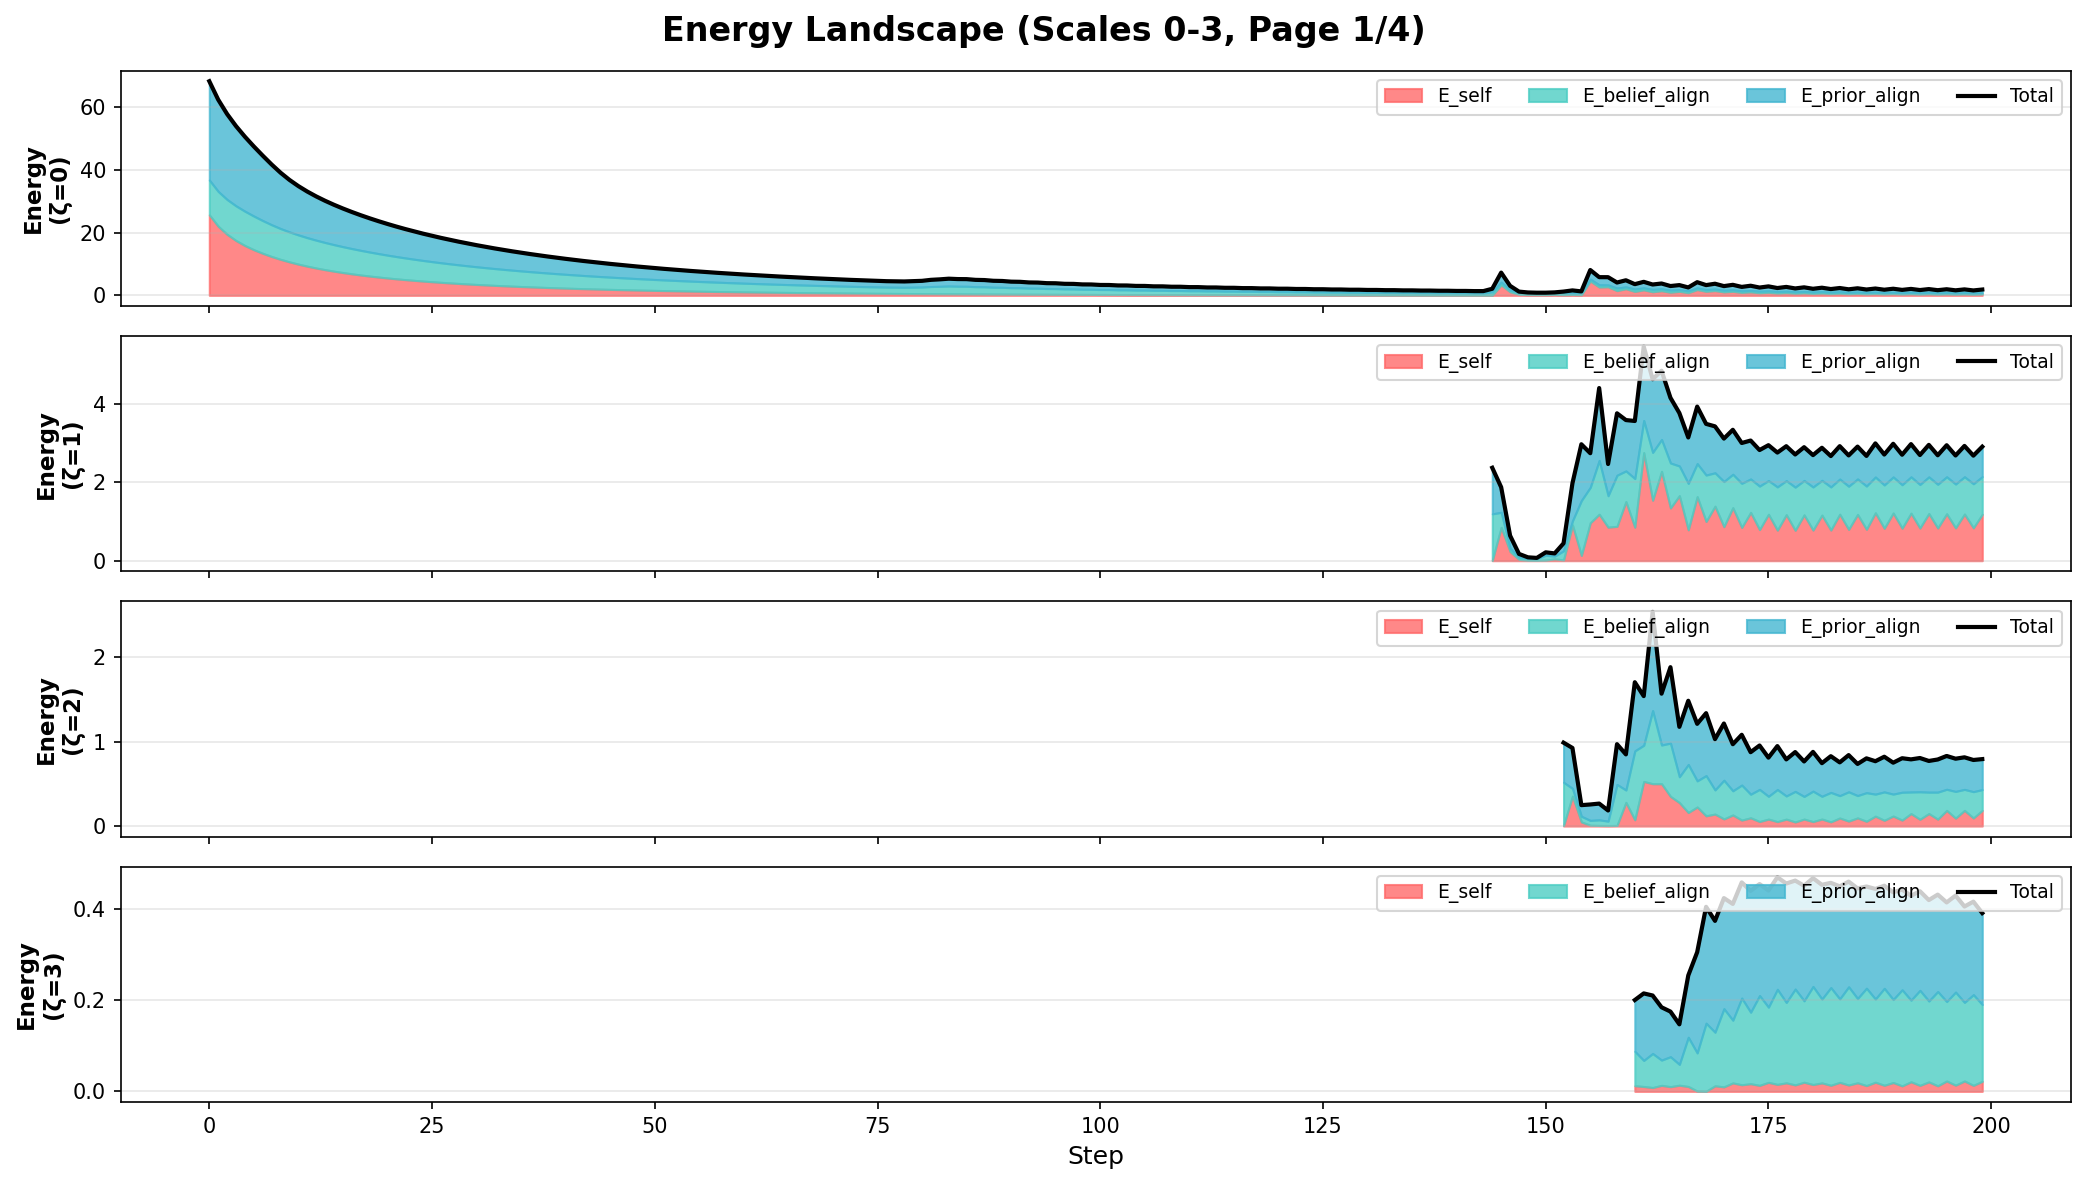
\includegraphics[width=0.8\linewidth]{Fig_5.png}
\caption{Mass-precision relationship validation. \textbf{(A)} Measured inertial mass versus prior precision showing $R^2 = 0.9998$ agreement with the theoretical prediction $M \propto \Lambda_p$. \textbf{(B)} Frequency scaling: oscillation frequency varies as $\omega \propto \sqrt{k/M}$, confirming harmonic oscillator behavior with precision-dependent mass. Error bars represent standard deviation over 10 independent simulations.}
\label{fig:mass_precision}
\end{figure}

The measured mass scales linearly with prior precision ($R^2 = 0.9998$), confirming the core theoretical prediction. Oscillation frequencies follow $\omega \propto \sqrt{k/M}$ as expected for harmonic motion with precision-dependent mass.

\subsection{Underdamped Versus Overdamped Dynamics}

Figure~\ref{fig:dynamics} contrasts underdamped Hamiltonian dynamics (preserving the full second-order structure) with overdamped gradient flow (standard active inference). The underdamped system exhibits oscillation, overshooting, and resonance phenomena absent in gradient flow. Phase portraits reveal closed orbits (energy conservation) in the underdamped case versus monotonic approach to equilibrium in the overdamped case.

\begin{figure}[t]
\centering
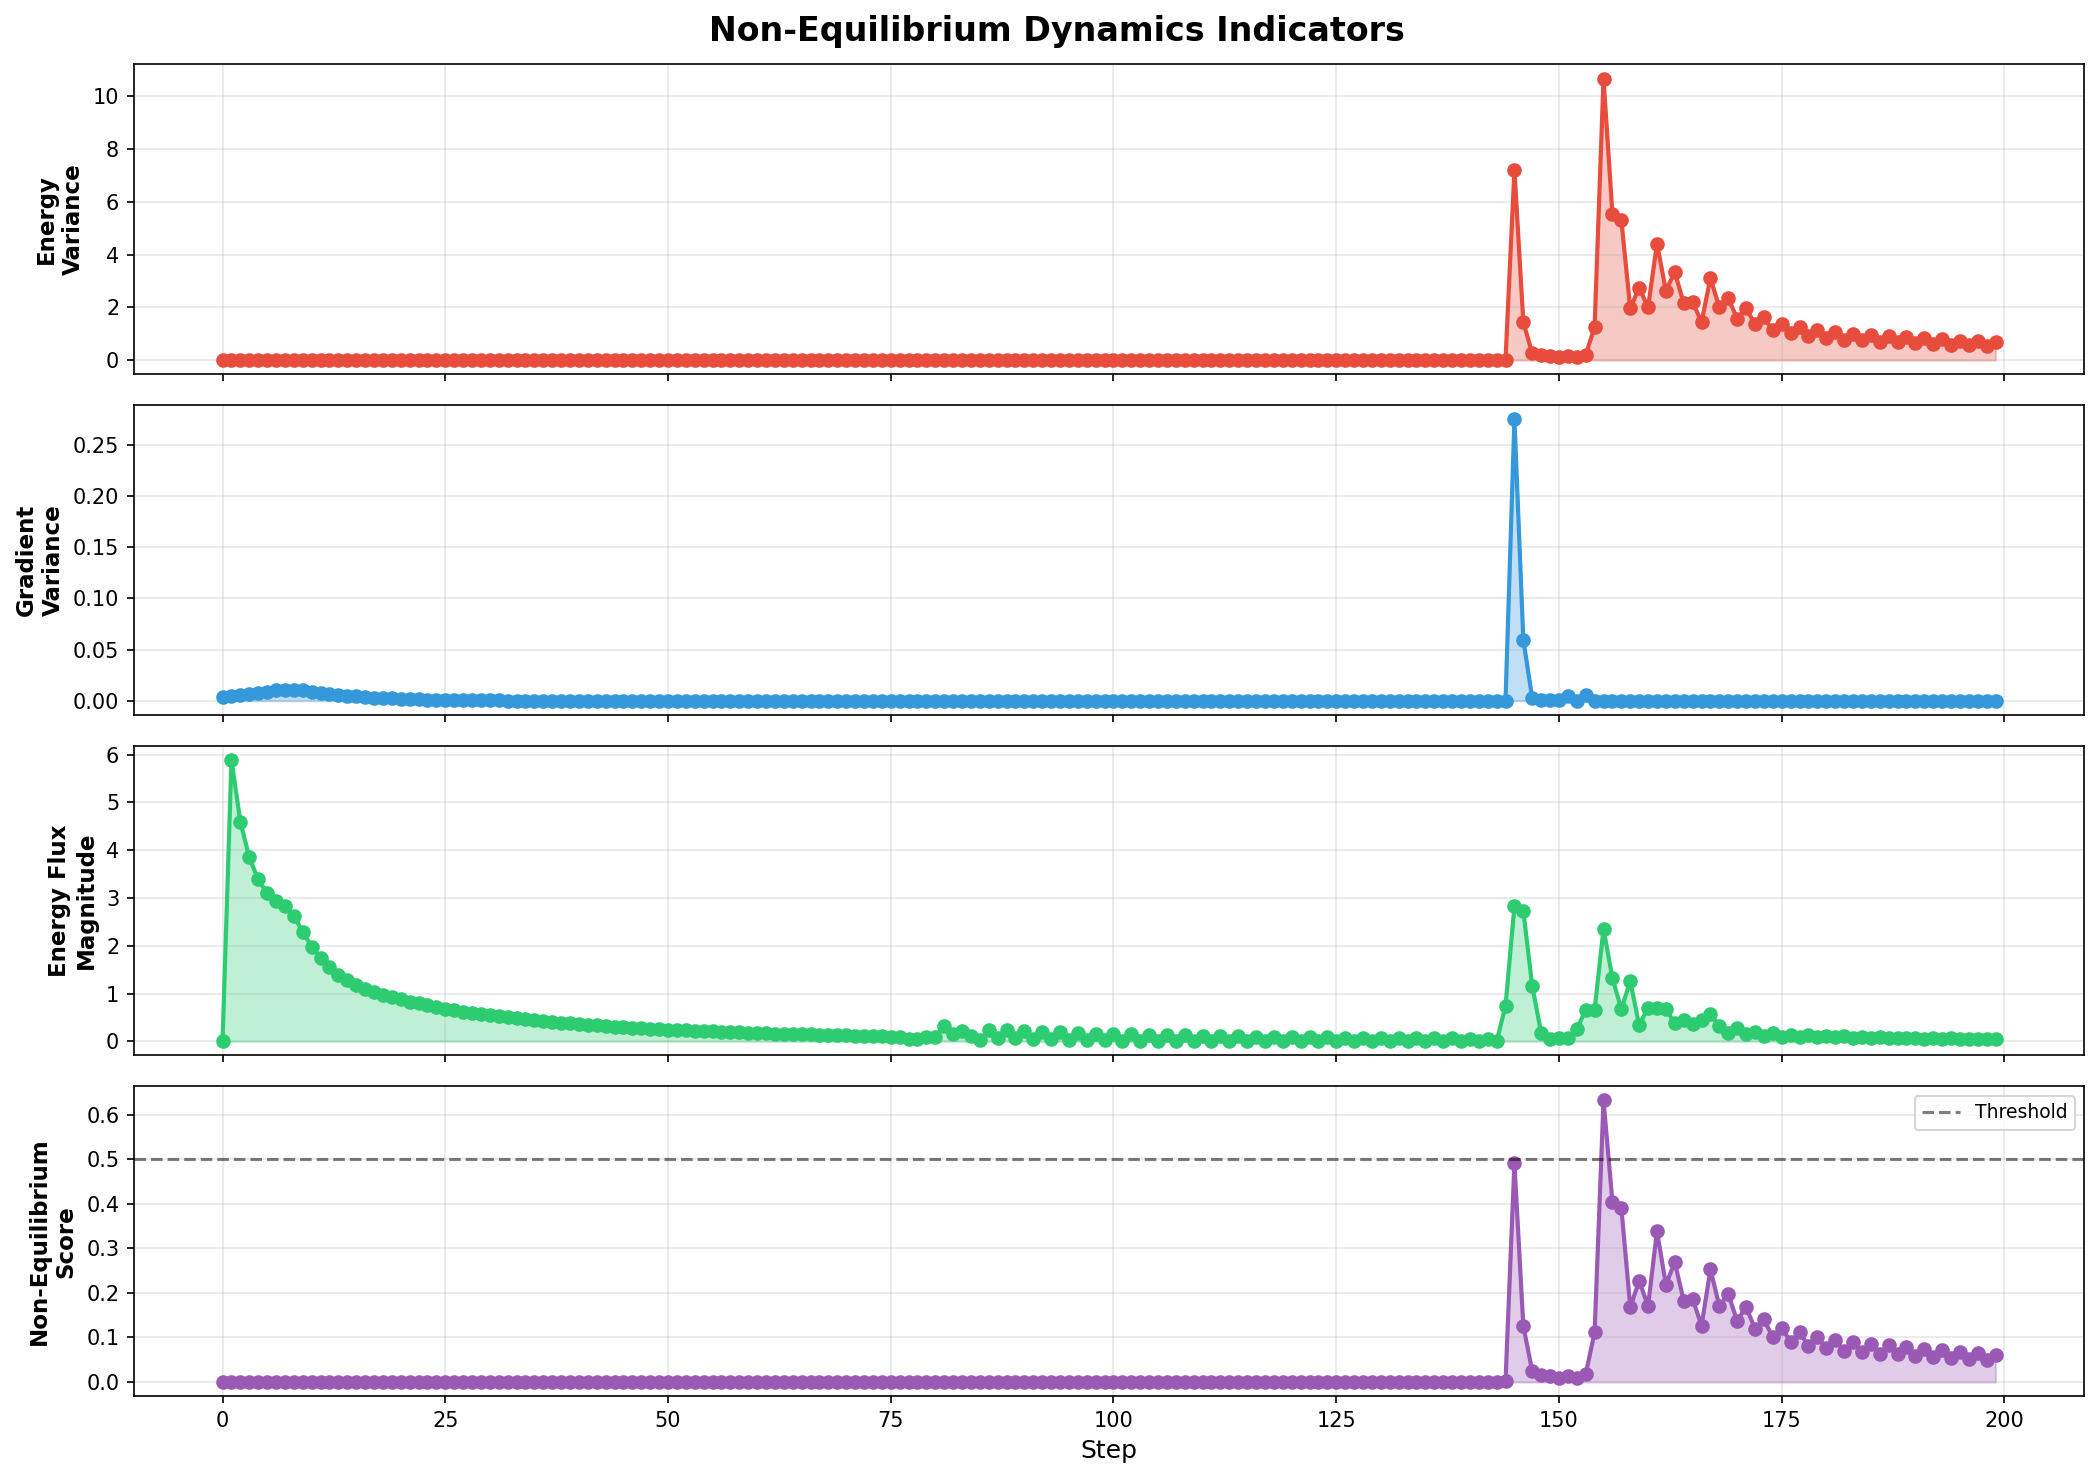
\includegraphics[width=0.8\linewidth]{Fig_6.png}
\caption{Underdamped versus overdamped dynamics. \textbf{Left:} Belief trajectories showing oscillatory approach to equilibrium (underdamped, blue) versus monotonic convergence (overdamped, orange). \textbf{Right:} Phase portraits revealing closed orbits (energy conservation) in the Hamiltonian system versus spiral approach in the damped system.}
\label{fig:dynamics}
\end{figure}

\subsection{Information-Geometric Proper Time}
\label{sec:proper_time}

Agents with different prior precisions accumulate different proper times along their belief trajectories:
\begin{equation}
\Delta\tau_i = \int_{\tau_1}^{\tau_2}\sqrt{g_{\mathcal{B}}(\dot{q}_i, \dot{q}_i)}\,d\tau
\end{equation}

We describe this as \emph{information-geometric time dilation}---agents with higher mass (greater precision) traverse longer paths in the statistical manifold and accumulate more Fisher-Rao arc length. This is geometrically interesting but distinct from relativistic time dilation: the quantitative structure differs from special/general relativity, and recovering Lorentz-type transformations remains an open problem. The effect demonstrates that the framework produces observer-dependent temporal structure from information geometry, though connecting this to physical proper time requires resolving the Lorentzian signature problem (Section~\ref{sec:lorentzian}).

\begin{figure}[t]
\centering
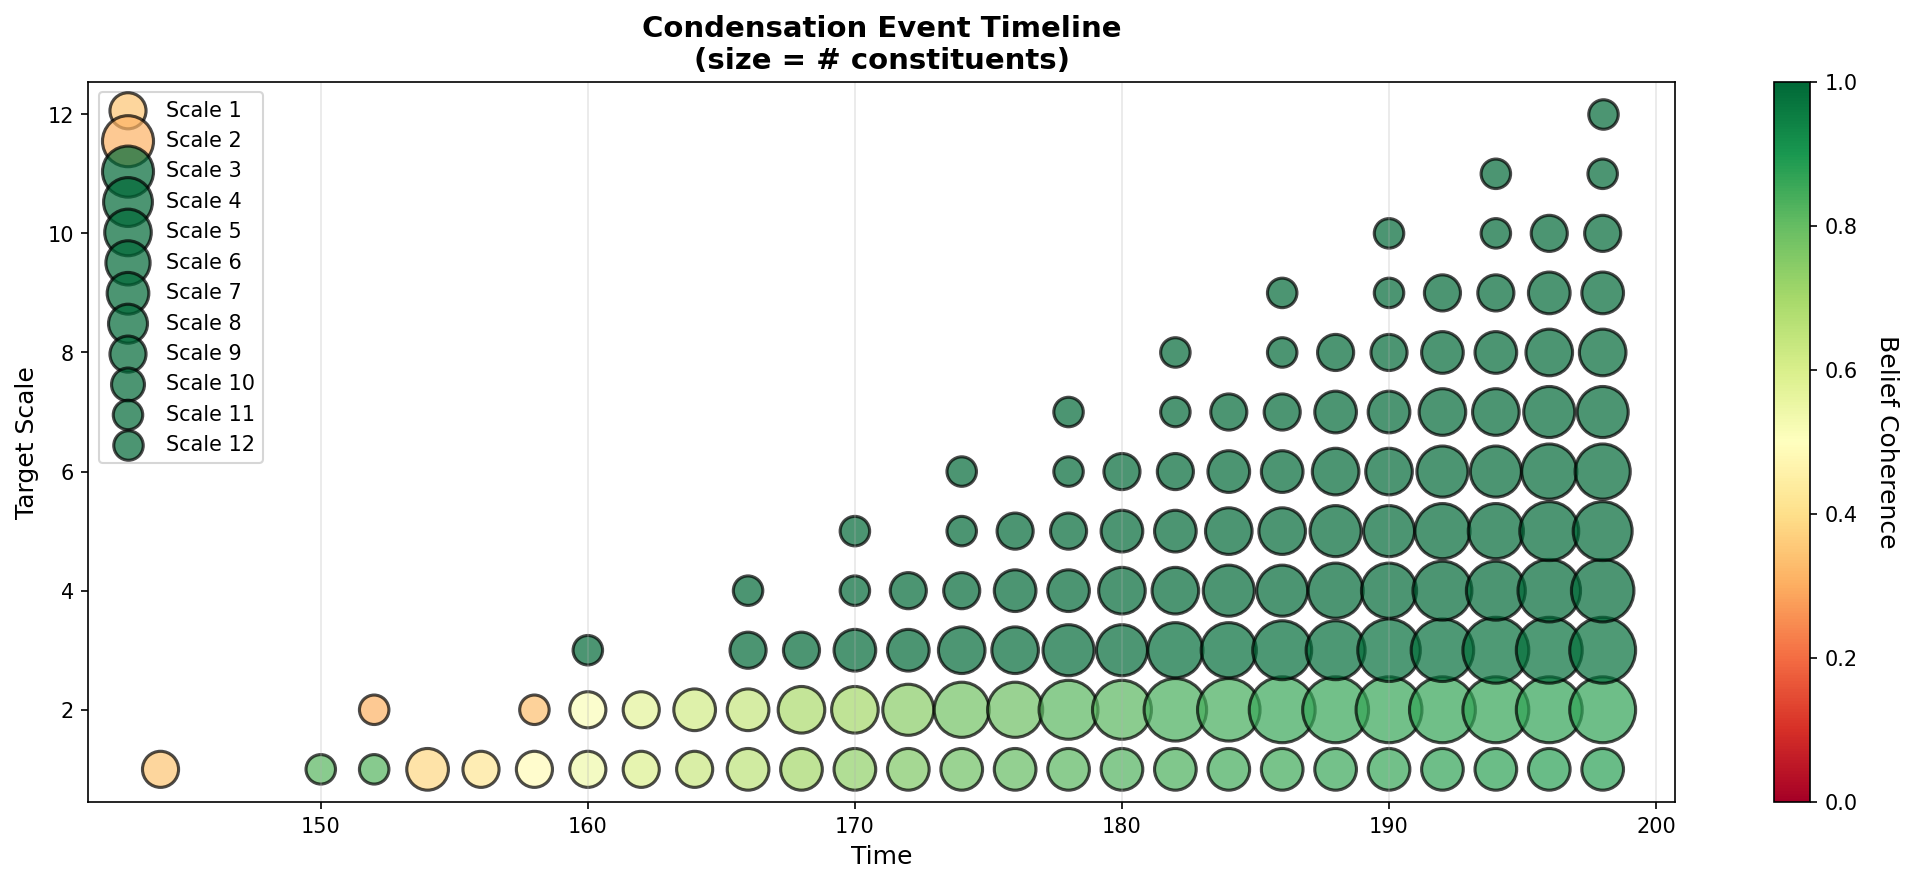
\includegraphics[width=0.8\linewidth]{Fig_7.png}
\caption{Information-geometric proper time dilation. Agents with different prior precisions (masses) accumulate different proper times. Higher-precision agents traverse longer paths in the statistical manifold. This represents precision-dependent proper time, not genuine relativistic time dilation---the quantitative structure differs from special/general relativity.}
\label{fig:proper_time}
\end{figure}

\subsection{Meta-Agent Emergence}

We conducted emergence experiments with 8 base agents across 13 dimensions, with consensus checks every 2 steps and a 25-level hierarchy cap. No hierarchical structure was imposed---all emergence was spontaneous.

The system evolved through three phases: \textbf{Phase I} (steps 0--140): local free energy minimization with agents optimizing individually; \textbf{Phase II} (steps 140--160): critical transition with rapid hierarchical condensation; \textbf{Phase III} (steps 160--200): hierarchical structure stabilizing across multiple scales.

\begin{figure}[t]
\centering
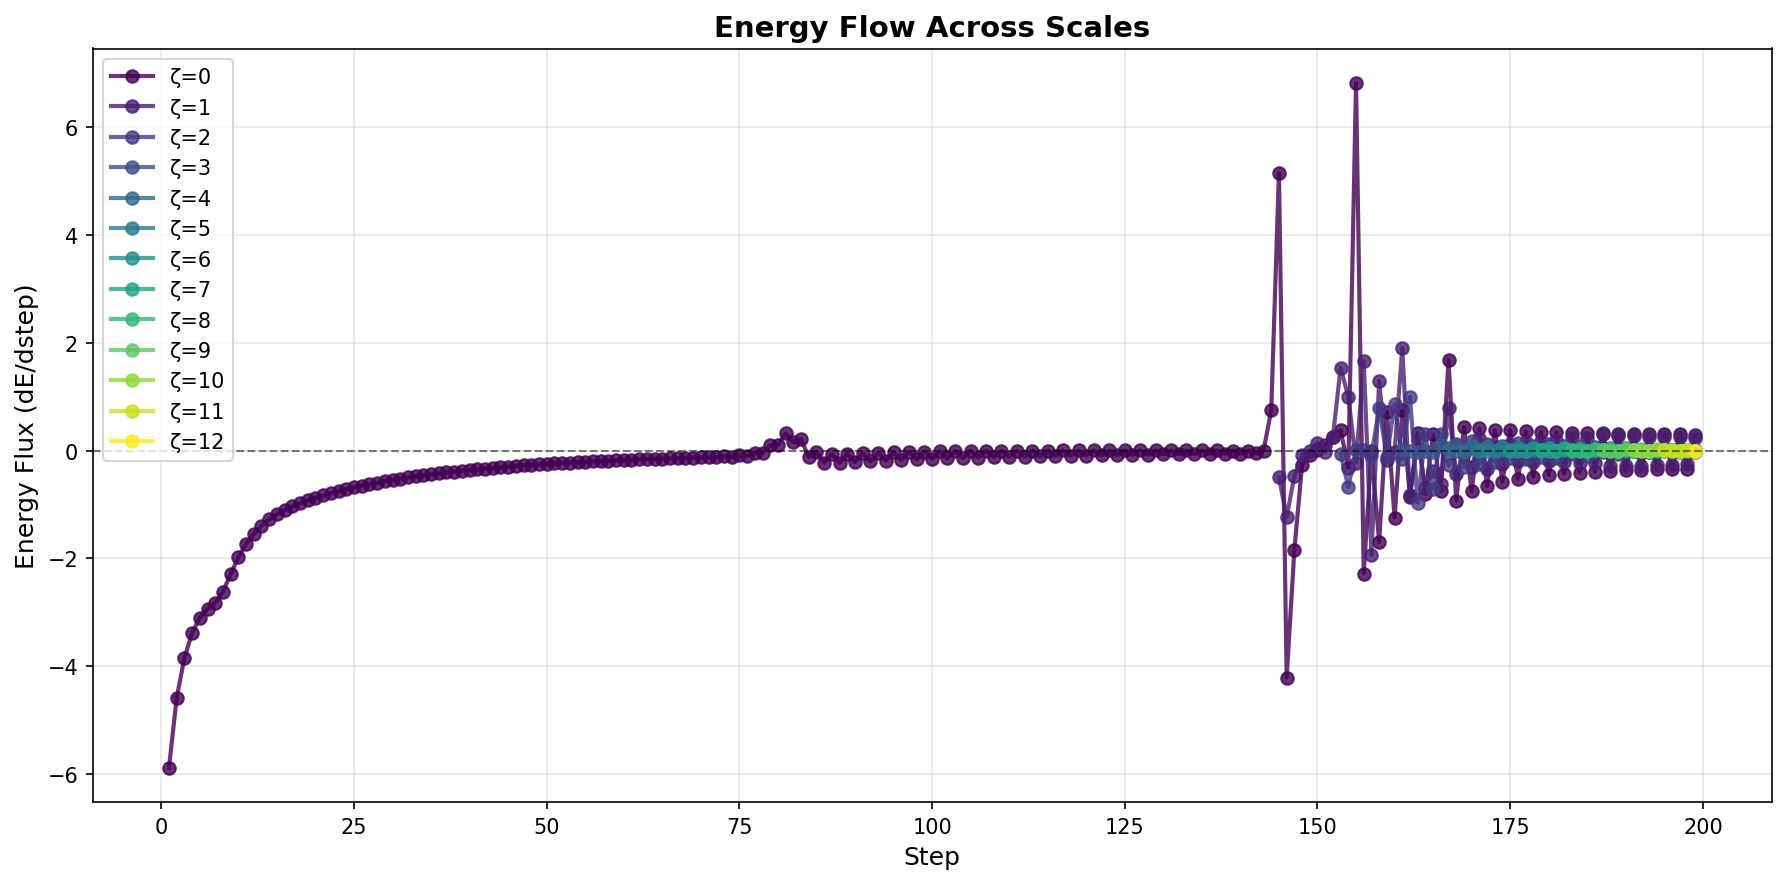
\includegraphics[width=0.8\linewidth]{Fig_4.png}
\caption{Meta-agent emergence across hierarchical scales. Energy components and hierarchical structure evolve through three phases: independent optimization (I), critical transition (II), and hierarchical condensation (III). No structure was imposed---all emergence is spontaneous from variational free energy minimization.}
\label{fig:emergence}
\end{figure}

The final architecture exhibited 13 hierarchical scales with bidirectional information flow validated through non-zero mutual information $\mathcal{I}_{s \to s+1} > 0$ at each scale transition. Energy conservation was maintained to machine precision under symplectic integration.

%==============================================================================
\section{Emergent Geometry: The Pullback Construction}
\label{sec:pullback}
%==============================================================================

\subsection{From Information to Geometry}

Wheeler's ``it from bit'' proposes that physical reality derives from information. We demonstrate how geometric structure emerges through pullback of Fisher-Rao metrics from statistical manifolds to the base space.

Each agent's belief section $\sigma_i^{(q)}: \mathcal{C} \to E_q$ induces a metric on $\mathcal{C}$:
\begin{equation}
\boxed{G^{(q)}_{i,\mu\nu}(c) = \mathbb{E}_{q_i(c)}\left[(\partial_\mu\log q_i)(\partial_\nu\log q_i)\right]}
\label{eq:pullback_belief}
\end{equation}

Similarly, the prior section induces:
\begin{equation}
\boxed{G^{(p)}_{i,\mu\nu}(c) = \mathbb{E}_{p_i(c)}\left[(\partial_\mu\log p_i)(\partial_\nu\log p_i)\right]}
\label{eq:pullback_prior}
\end{equation}

These metrics measure how rapidly statistical fields vary across $\mathcal{C}$. The induced metric encodes information-theoretic structure as geometric structure---this is the precise mathematical realization of Wheeler's vision.

\subsection{Dual Geometries}

The belief pullback $G_i^{(q)}$ encodes \emph{epistemic geometry}---highly dynamical, reflecting current posterior beliefs. The prior pullback $G_i^{(p)}$ encodes \emph{ontological geometry}---quasi-static, reflecting the agent's generative model of reality. Different agents with different priors perceive different geometries on the same underlying $\mathcal{C}$.

For Gaussian agents on $\mathcal{C} = \mathbb{R}^2$ with isotropic covariance $\Sigma_i = \sigma^2 I$:
\begin{equation}
G^{(q)}_{i,\mu\nu}(c) = \frac{1}{\sigma^2}(\partial_\mu\mu_i)\cdot(\partial_\nu\mu_i)
\end{equation}
a conformal metric where high certainty (small $\sigma$) magnifies distances.

\subsection{Collective Geometry and Gauge Invariance}

The gauge-invariant consensus metric averages over gauge orbits:
\begin{equation}
\bar{G}_{\mu\nu}^{\mathrm{consensus}}(c) = \sum_i w_i(c)\langle G_i\rangle_{\mu\nu}(c), \qquad \langle G_i\rangle_{\mu\nu} = \int_G dg\,G_{i,\mu\nu}(c; \phi_i \to \phi_i + g)
\end{equation}

This construction is gauge-invariant by design and represents the closest analog to ``objective reality'' in the framework.

\subsection{Dimensional Structure}

The induced metric admits spectral decomposition $G_i(c) = \sum_a\lambda_a(c)(e_a \otimes e_a)$. Large eigenvalues indicate observable dimensions with rapid belief variation; small eigenvalues indicate dark dimensions carrying negligible information flux.

\subsection{The Lorentzian Signature Problem}
\label{sec:lorentzian}

The induced metrics are Riemannian (positive-definite) because they arise from the Fisher-Rao metric. Physical spacetime requires Lorentzian signature $(-,+,+,+)$. This is not a minor technical detail but the central unsolved challenge.

\textbf{The problem:} Fisher-Rao metrics are intrinsically positive-definite. No amount of agent dynamics within the current framework can produce indefinite signature through pullback.

\textbf{Proposed approaches and their prospects:}
\begin{enumerate}
\item \textbf{Gauge holonomy / Berry phases:} Non-zero field strength $F_{\mu\nu}$ might induce effective signature change through path-dependent transport. \emph{Status:} Suggestive but undemonstrated; holonomy is real-valued for $\mathrm{SO}(N)$, complicating sign changes.

\item \textbf{Cross-bundle morphisms:} Maps $\Phi: E_p \to E_q$ between prior and belief bundles might carry signature structure if constructed to distinguish temporal from spatial directions. \emph{Status:} Mathematically natural but no concrete mechanism identified.

\item \textbf{Emergent coarse-graining:} Lorentzian signature might emerge only at macroscopic scales through coarse-graining, remaining Riemannian microscopically. \emph{Status:} The most physically plausible route, but requires showing how coarse-graining produces sign changes.

\item \textbf{Unitary groups $\mathrm{SU}(N)$:} Replacing $\mathrm{SO}(N)$ with $\mathrm{SU}(N)$ introduces complex phases. The imaginary parts of Hermitian metrics can have indefinite signature. \emph{Status:} Most promising technically; $\mathrm{SU}(2)$ is the double cover of $\mathrm{SO}(3)$ and naturally introduces quantum-like structure.

\item \textbf{Non-commutative geometry / complex amplitudes:} Replacing classical probability distributions with complex-valued amplitudes fundamentally changes the metric structure. \emph{Status:} Requires developing the entire framework in a quantum setting, which has not been done.
\end{enumerate}

\textbf{What a solution requires:} Any resolution must (a) produce indefinite signature from information-geometric principles without ad hoc sign assignments, (b) recover $(-,+,+,+)$ specifically (not arbitrary signatures), and (c) be consistent with the rest of the framework's gauge structure. Without such resolution, claims about emergent spacetime remain mathematical analogy rather than physical explanation.

\subsection{Gauge Group Choice and Extensions}
\label{sec:gauge_choice}

Both manuscripts in the original development default to $G = \mathrm{SO}(N)$ without discussing alternatives. The choice has consequences for the mass formula and signature problem.

\textbf{$\mathrm{SO}(N)$} (current choice): Real orthogonal rotations of internal frames. Transport preserves real-valued precisions. The mass matrix is real symmetric. Provides physical interpretability through familiar spatial rotations. Cannot produce complex phases needed for quantum structure.

\textbf{$\mathrm{SU}(N)$}: Introduces complex phases through unitary transformations. Transport operators $\Omega_{ij} \in \mathrm{SU}(N)$ act as $\mu \mapsto \Omega_{ij}\mu$ with $\mu \in \mathbb{C}^N$. The mass formula generalizes: $\tilde{\Lambda}_{q_k} = \Omega_{ik}\Lambda_{q_k}\Omega_{ik}^\dagger$ with $\dagger$ replacing transpose. The Hermitian metric $g_{\mu\nu} = \mathrm{Re}\,\mathbb{E}[(\partial_\mu\log q)(\partial_\nu\log q)^*]$ admits indefinite signature through imaginary cross-terms. This connects directly to the Lorentzian signature problem.

\textbf{$\mathrm{U}(1)$}: The electromagnetic gauge group. Agents acquire phases $e^{i\theta_i}$ that multiply beliefs. Attention weights become $\beta_{ij} \propto \exp[-\kappa^{-1}\mathrm{KL}(q_i \| e^{i(\theta_i - \theta_j)}q_j)]$, introducing interference effects absent in $\mathrm{SO}(N)$.

The framework's mathematical structure accommodates any compact Lie group $G$ without modification to the variational principle. The choice of $G$ determines which physical phenomena the framework can model. Extension to $\mathrm{SU}(N)$ is the most promising direction for resolving both the signature problem and quantum connections.

%==============================================================================
\section{Participatory Hierarchy and Transformer Validation}
\label{sec:hierarchy}
%==============================================================================

\subsection{Multi-Scale Participatory Structure}

Meta-agents form when scale-$s$ agents achieve sufficient coherence. The consensus score $\Gamma(\{i\}, c) = C_{\mathrm{belief}} \cdot C_{\mathrm{model}} \cdot P(\{i\}, c)$ combines belief coherence, model coherence, and spatial overlap. Meta-agent beliefs are constructed via gauge-covariant weighted averaging of transported constituent beliefs.

The participatory loop closes through top-down information flow: a meta-agent $I$'s belief becomes the prior for constituent agents via $p_i^{(s)}(c) = \Omega_{i,I}[q_I^{(s+1)}](c)$. This creates Wheeler's ``self-excited circuit''---constituents inform meta-agents through their beliefs, while meta-agents shape constituent expectations through prior propagation.

The free energy at scale $(s+1)$ has the same functional form as at scale $s$, suggesting the framework may exhibit critical phenomena, fixed points, or universal behavior analogous to phase transitions.

\subsection{Empirical Validation: Transformer Emergence}
\label{sec:transformers}

Standard transformer architectures emerge as the zero-dimensional limit of our construction. When $\mathcal{C} \to$ finite token set and $G \to \{e\}$, transport becomes trivial and the attention weights reduce to:
\begin{equation}
\beta_{ij} = \frac{\exp[-\kappa^{-1}\mathrm{KL}(q_i \| q_j)]}{\sum_k\exp[-\kappa^{-1}\mathrm{KL}(q_i \| q_k)]}
\end{equation}

For Gaussian beliefs with small covariance differences, $\mathrm{KL}(q_i \| q_j) \approx -Q_i \cdot K_j + \mathrm{const}$, exactly matching standard scaled dot-product attention with $\kappa = \sqrt{d_k}$.

We implemented three architectures of increasing theoretical fidelity~\cite{Dennis2025transf}:

\begin{table}[h]
\centering
\small
\begin{tabular}{lccc}
\toprule
\textbf{Architecture} & \textbf{PPL ($\downarrow$)} & \textbf{Parameters} & \textbf{Key Feature} \\
\midrule
Standard baseline & 22.6 & 8,688 & Dot-product attention + MLP \\
Gauge attention & 22.36 & 8,688 & KL-based attention + MLP \\
Full Gauge VFE & \textbf{18.06} & \textbf{6,534} & Natural gradient on manifold \\
\bottomrule
\end{tabular}
\caption{WikiText-2 character-level results. The full gauge VFE achieves 20\% lower perplexity with 25\% fewer parameters, using no learned weight matrices---all computation is variational. The $r = 0.821$ correlation with BERT attention validates the information-theoretic coupling mechanism.}
\label{tab:transformer}
\end{table}

The full gauge VFE architecture achieves competitive performance despite using only geometric updates---natural gradient descent on statistical manifolds with no learned weight matrices, no multi-layer perceptrons, and no activation functions. Training curves (Figs.~\ref{fig:train_baseline}--\ref{fig:train_vfe}) show stable convergence with excellent generalization (train-validation gap $< 0.1$ bits-per-character).

Computational overhead is severe (825$\times$ slower than optimized dot-product attention), reflecting first-generation implementation prioritizing mathematical fidelity over efficiency. This overhead is not fundamental---standard transformers are efficient approximations to the underlying gauge-theoretic structure, paralleling how Newtonian mechanics is computationally simpler than relativistic mechanics.

\begin{figure}[t]
\centering
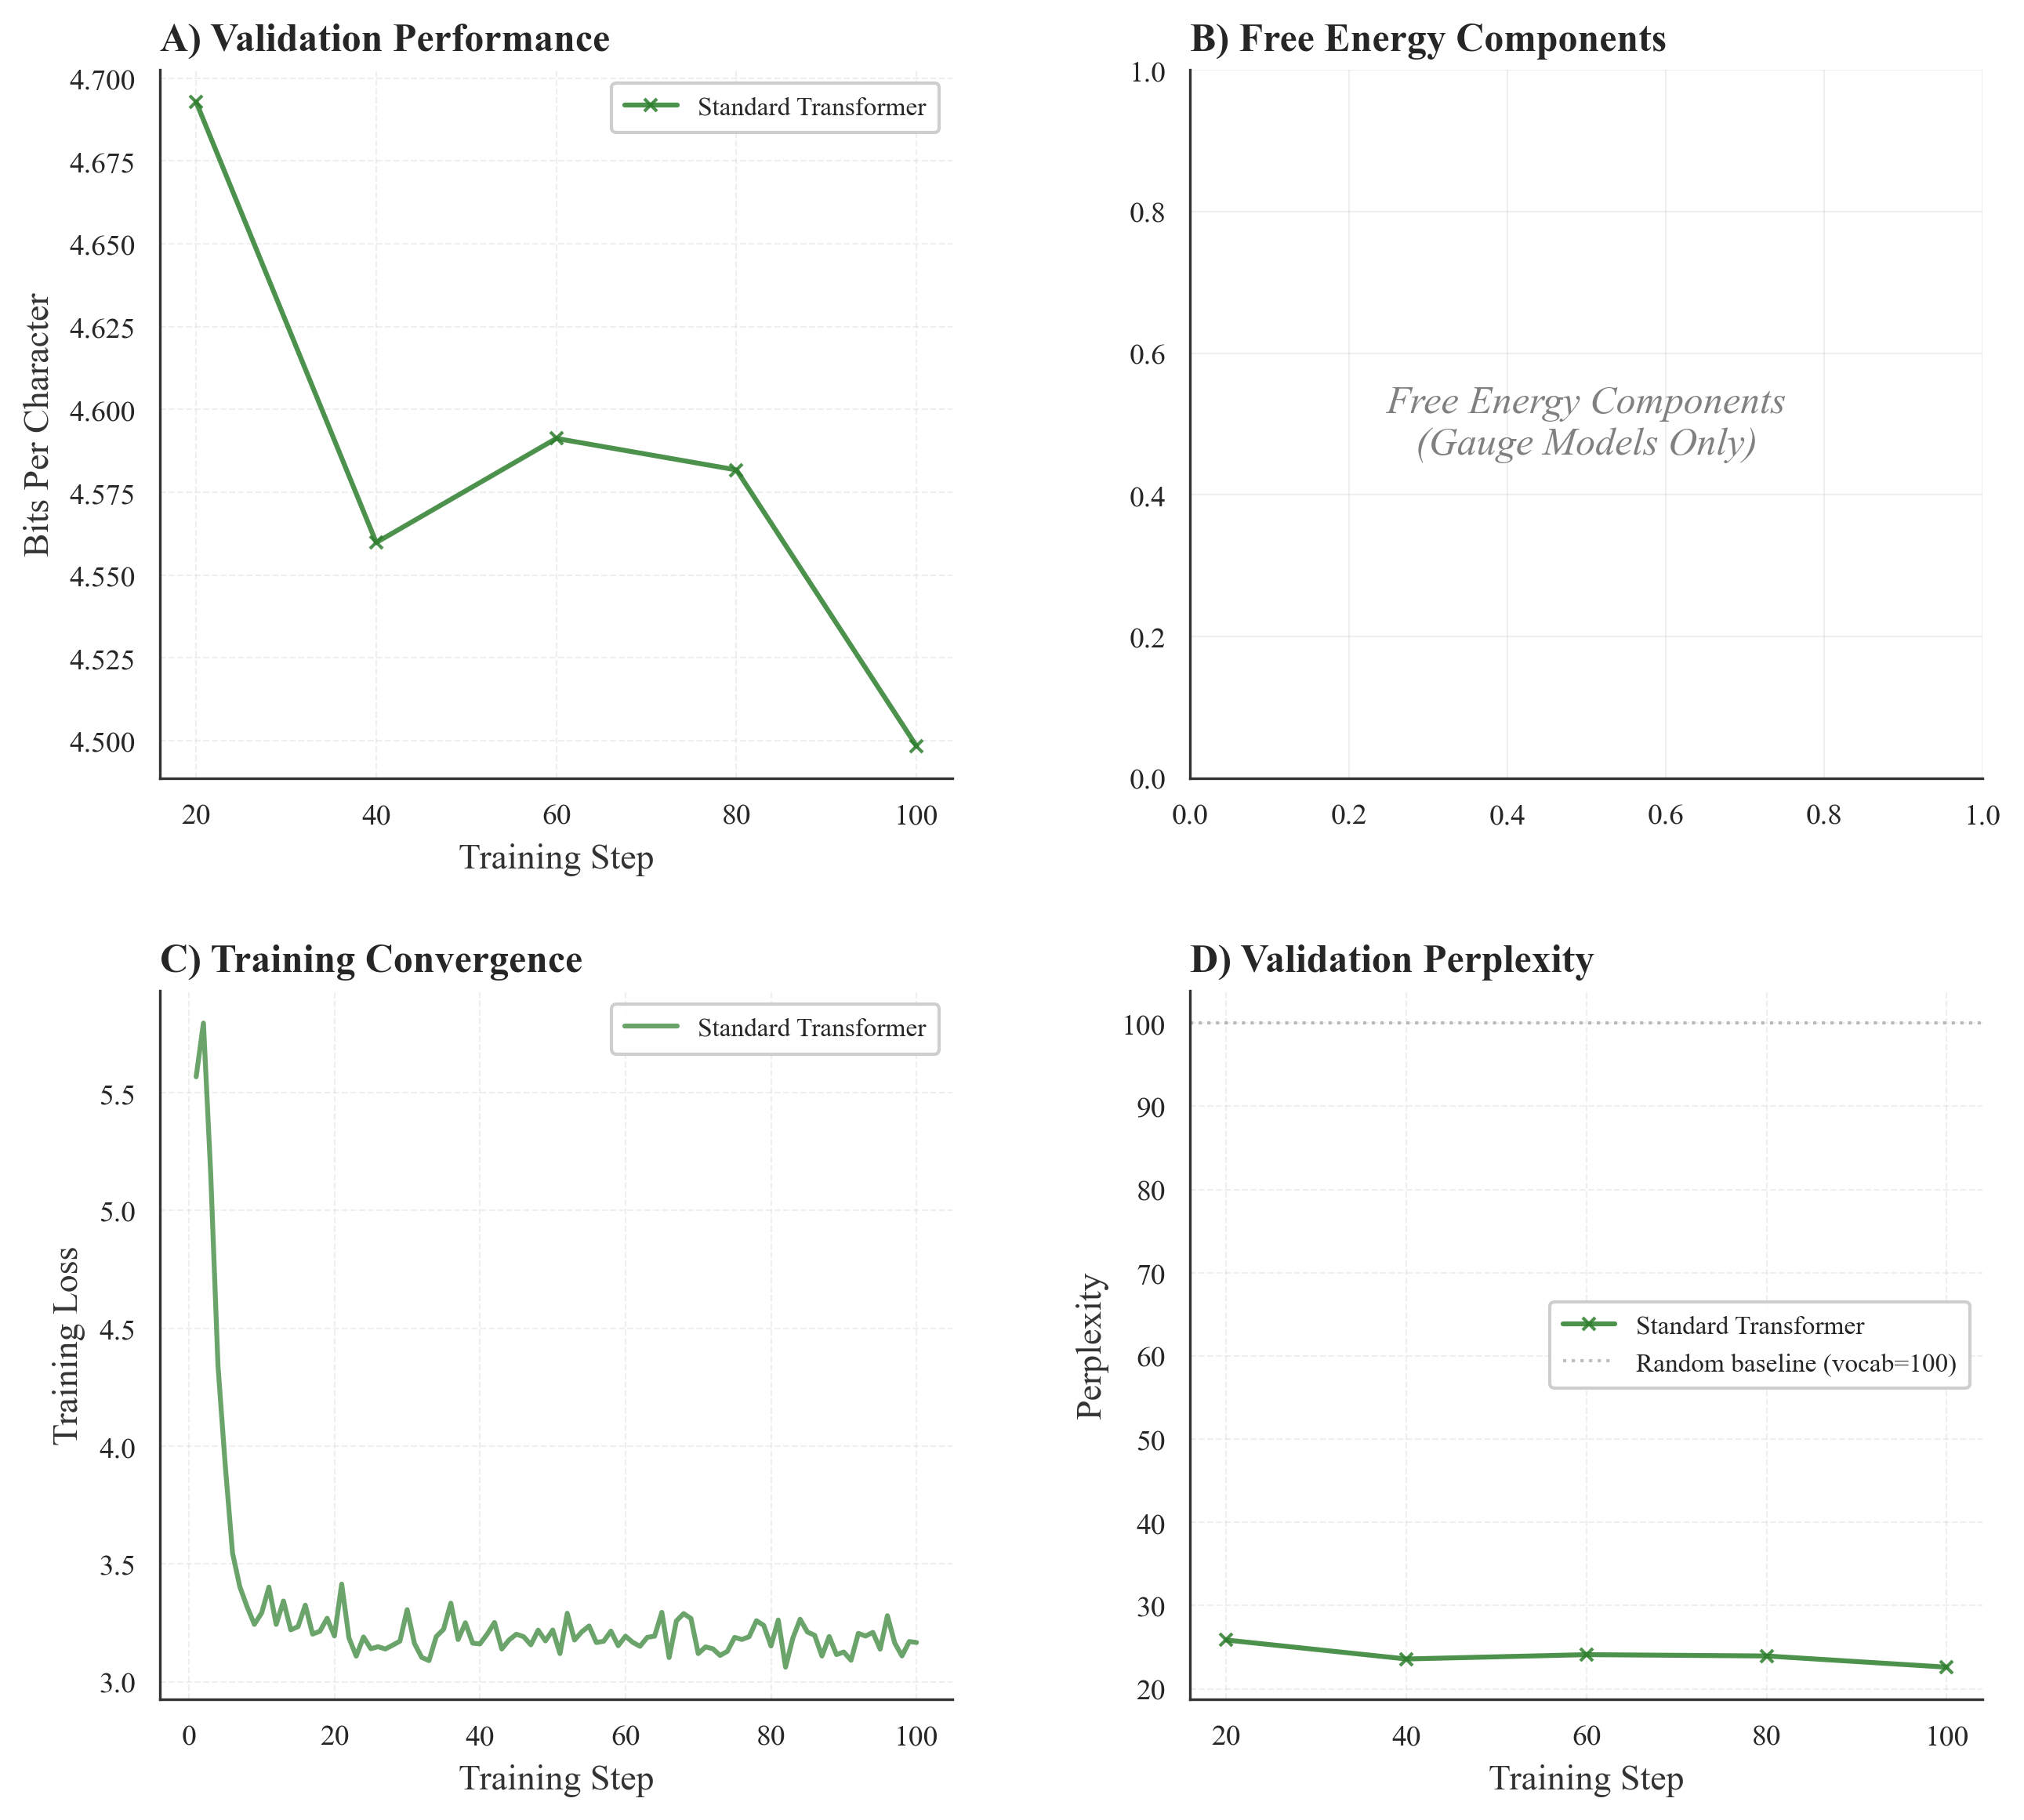
\includegraphics[width=0.32\linewidth]{Fig_9.png}
\hfill
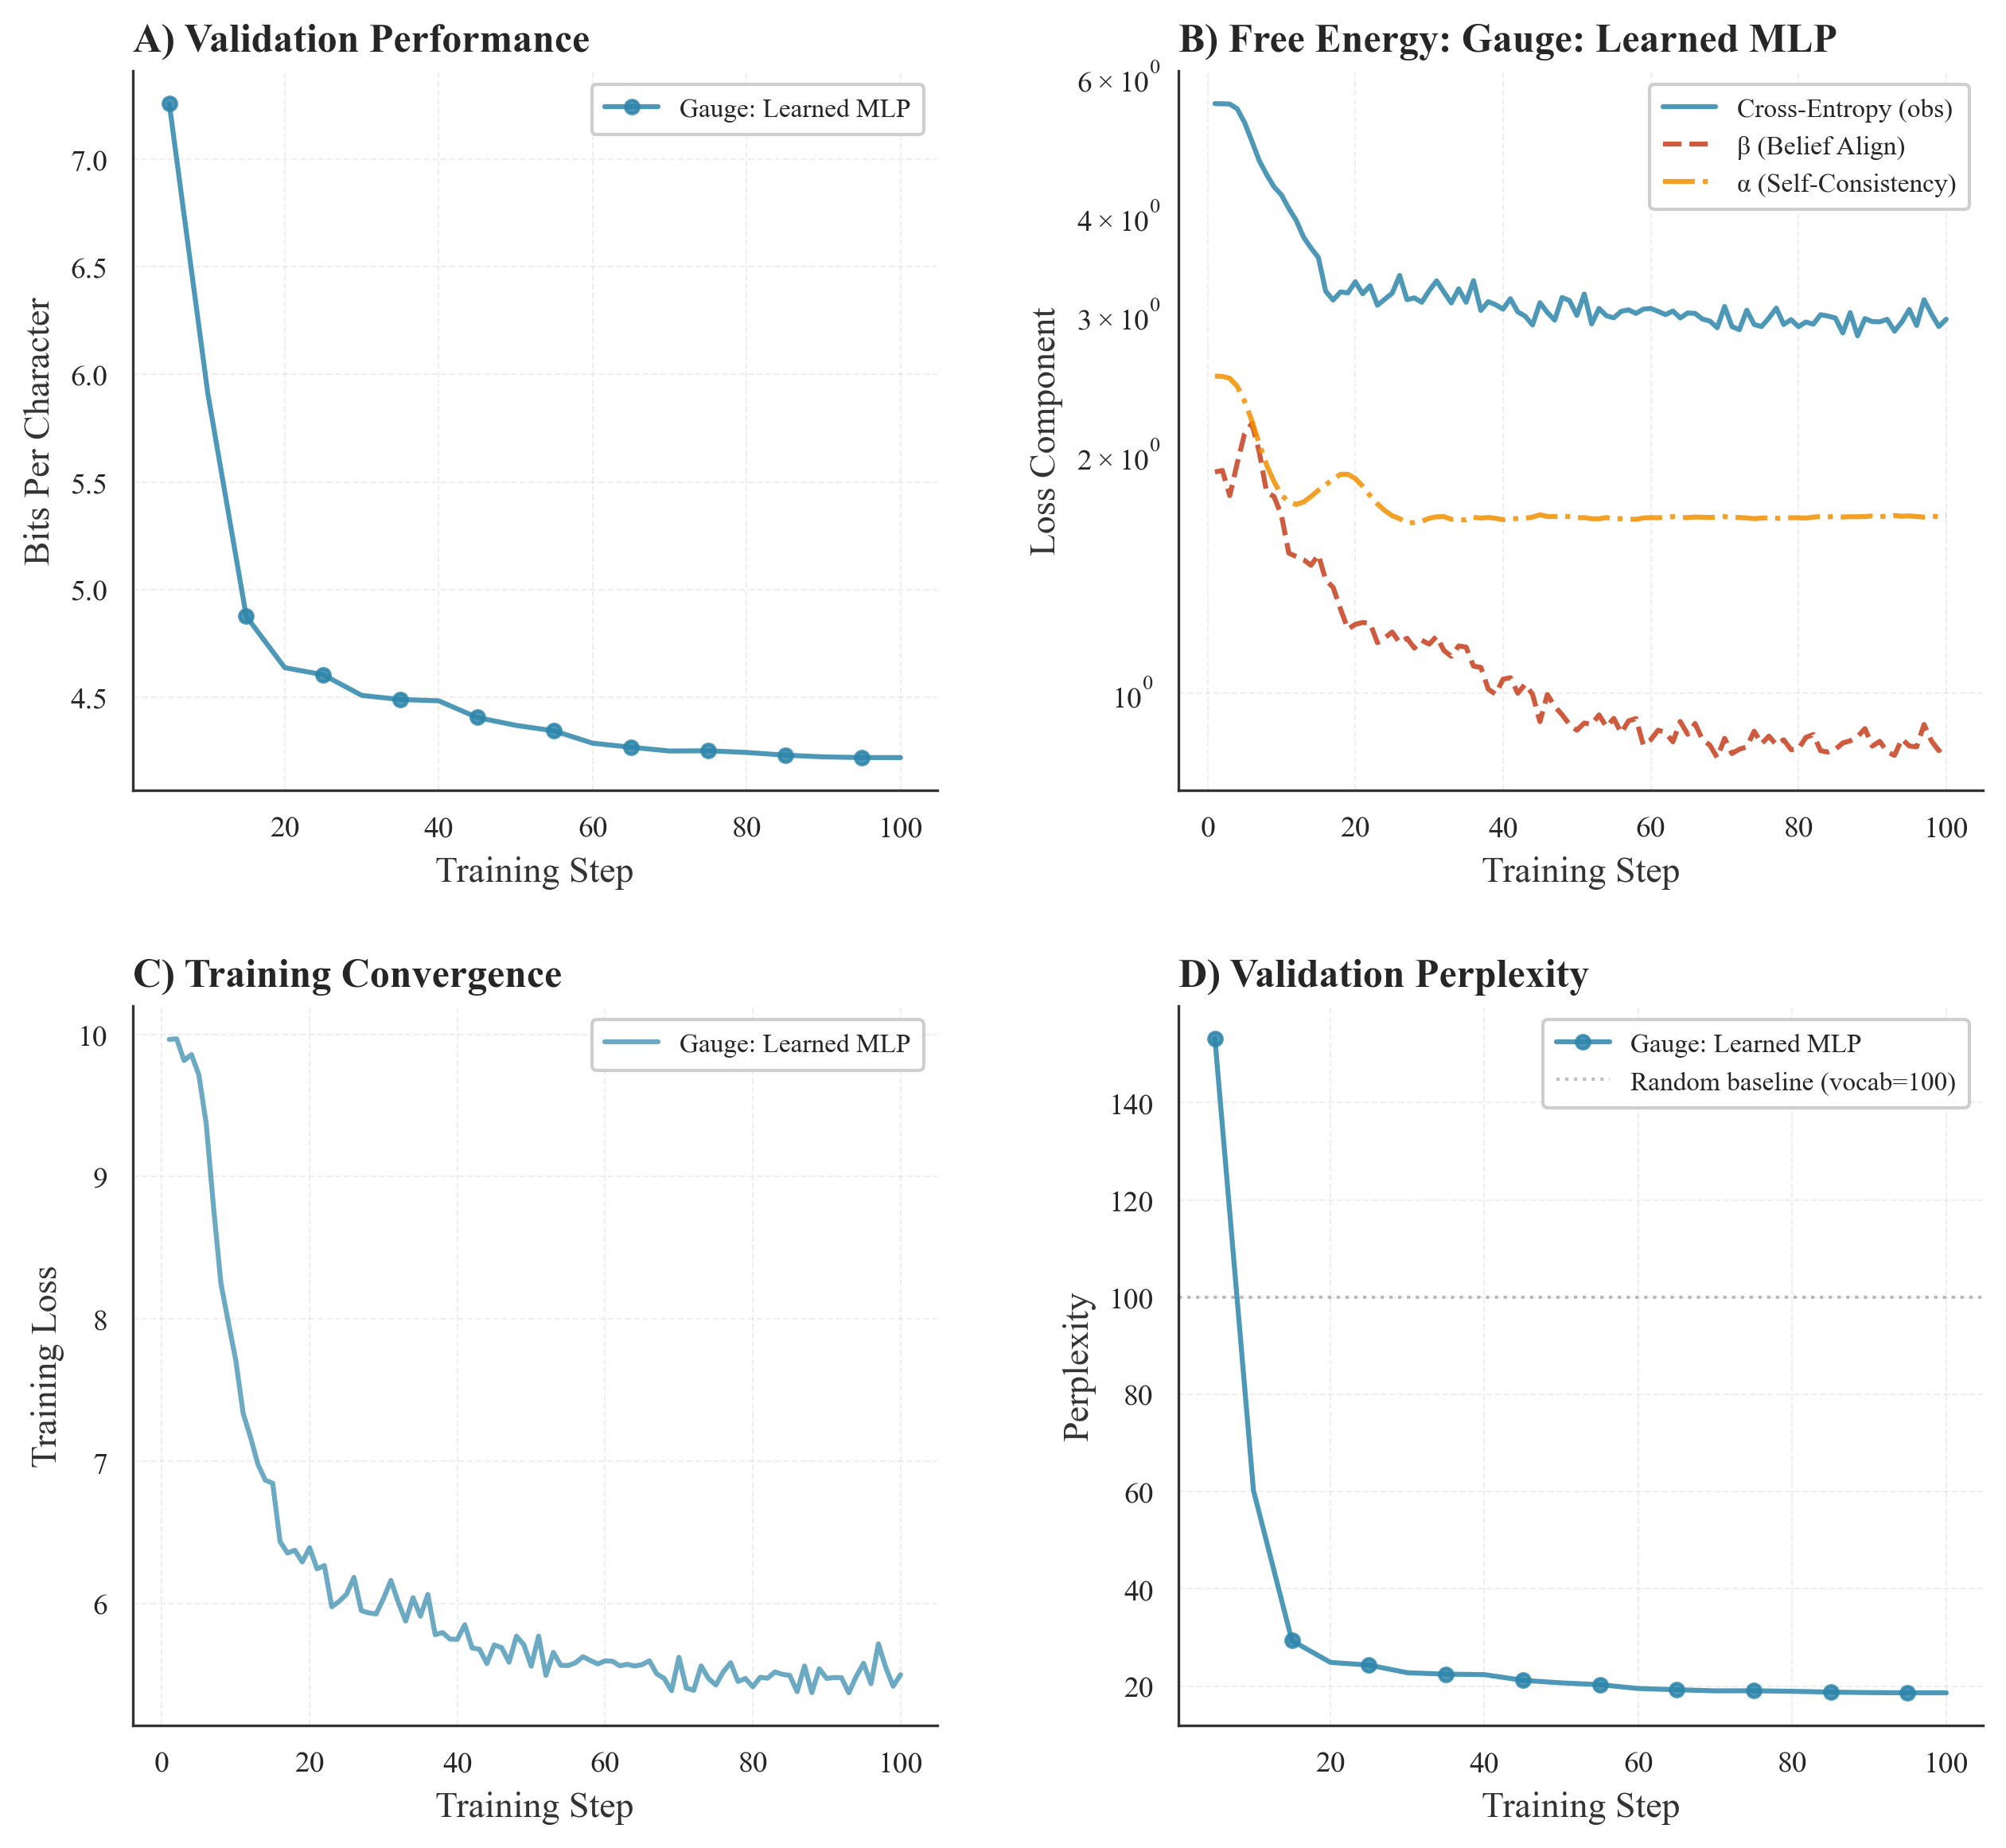
\includegraphics[width=0.32\linewidth]{Fig_10.png}
\hfill
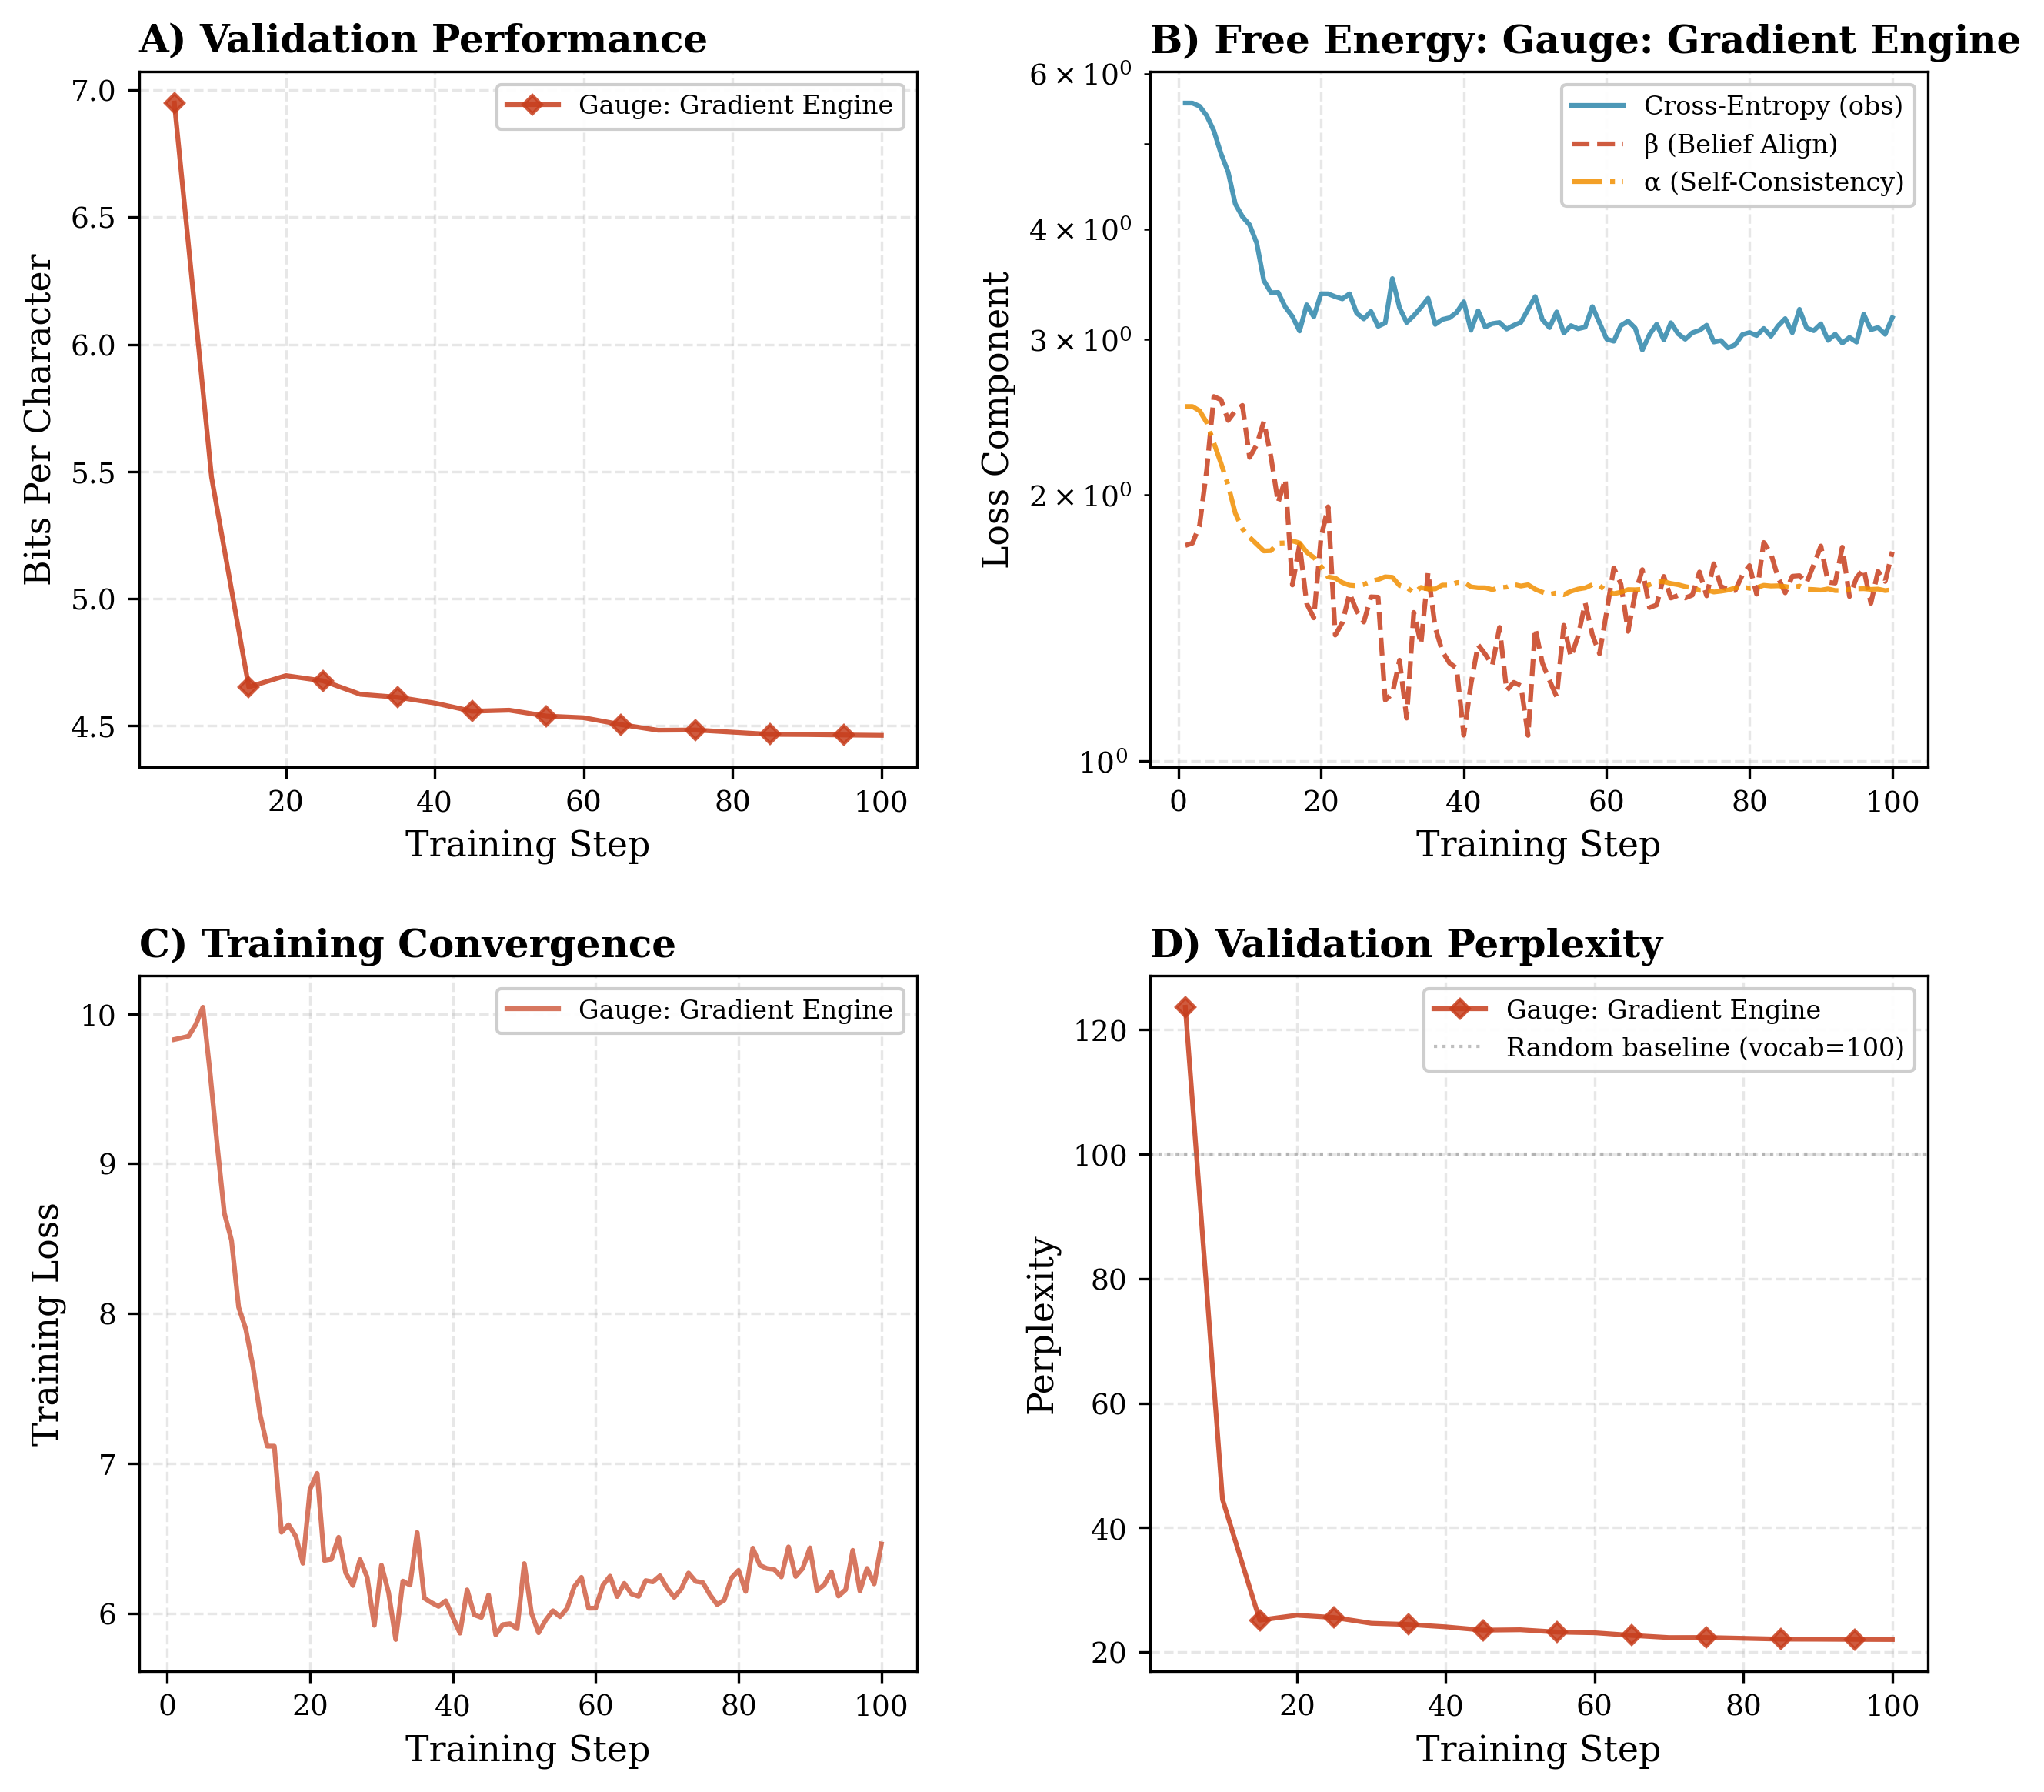
\includegraphics[width=0.32\linewidth]{Fig_11.png}
\caption{Training dynamics for all three architectures. \textbf{Left:} Standard baseline (PPL 22.6). \textbf{Center:} Gauge attention (PPL 22.36). \textbf{Right:} Full Gauge VFE (PPL 18.06). All show stable convergence; the gauge VFE achieves lowest loss despite using only geometric updates.}
\label{fig:train_baseline}
\label{fig:train_gauge}
\label{fig:train_vfe}
\end{figure}

%==============================================================================
\section{Discussion}
\label{sec:discussion}
%==============================================================================

\subsection{Physical Interpretation}

Our framework unifies Wheeler's participatory universe, Friston's Free Energy Principle, gauge theory, and transformer architectures. The central physical insight is that the Hessian of variational free energy provides a natural inertial mass tensor, with mass decomposing into prior, sensory, incoming social, and outgoing recoil contributions. The overdamped limit recovers standard active inference, while the full second-order structure predicts oscillation, resonance, and information-geometric time dilation.

The kinetic term $\frac{1}{2}\dot{\mu}^T\Sigma^{-1}\dot{\mu}$ was previously ``missed'' because standard treatments employ first-order gradient descent, implicitly discarding the mass tensor. Neural systems may well operate in this overdamped regime. But the full second-order structure reveals physics-like dynamics hidden in the variational principle.

\subsection{Falsifiable Predictions}
\label{sec:predictions}

\subsubsection{Mass Deficit in Quantum Superpositions}

If the framework can be extended to quantum systems---which remains to be demonstrated---it would predict that a particle in spatial superposition has reduced inertial mass:
\begin{equation}
M_{\mathrm{superposition}} = \frac{1}{\sigma^2} \ll M_{\mathrm{localized}} = \frac{1}{\sigma_0^2}
\end{equation}

This prediction is \emph{conditional}: it rests on extending the classical-statistical framework to quantum systems, which has not been done. We retain the distinction from Penrose-Di\'osi gravitational decoherence~\cite{Penrose1996}: their framework predicts massive superpositions are \emph{unstable} (faster collapse), while ours would predict they have \emph{reduced mass} (more stable). Current levitated optomechanics experiments approach the required sensitivity~\cite{Bateman2014,Millen2020}. A null result would falsify the central claim that $M = \mathrm{tr}(\Sigma_p^{-1})$ in the quantum domain.

\subsubsection{Gauge Curvature in Language}

The strongest near-term testable prediction involves gauge curvature in linguistic systems. The field strength $F_{\mu\nu}$ measures path-dependence of information transport. We conjecture that linguistic evolution minimizes gauge curvature, measurable through: curvature changes in historical corpora, curvature differences between creoles and pidgins, and curvature reduction in developing scientific terminology. Unlike spacetime claims, linguistic curvature is directly measurable.

\subsection{Implications for Language and Cognition}

The transformer derivation reveals that language may be fundamentally a multi-agent coordination problem solved through information-theoretic coupling, with each token functioning as an agent maintaining beliefs, priors, and gauge frames. Syntactic structure may emerge from the geometry of information flow rather than being imposed by explicit rules.

\subsection{Consciousness and Hierarchical Integration}

The multi-scale framework provides formal structure for aspects of consciousness, though this remains highly speculative. Conscious systems may correspond to meta-agents maintaining representations of constituent agents, with self-awareness as recursive meta-representation and qualia as gauge-frame-dependent phenomenology. These interpretations provide mathematical vocabulary without necessarily explaining why information geometry produces felt quality.

\subsection{Open Problems}
\label{sec:open_problems}

\textbf{Lorentzian signature} (Section~\ref{sec:lorentzian}): The most critical unsolved problem. Without resolution, spacetime claims remain analogy.

\textbf{Dimensional analysis:} Rigorous conversion between information-theoretic and physical units is lacking. Deriving even one dimensionless constant from information geometry would constitute major progress.

\textbf{Scaling:} Our largest validated system (8 agents, dimension 13) is tiny. Phase transitions, critical phenomena, and behavior at $N > 1000$ are unknown.

\textbf{Quantum extension:} The framework operates with classical distributions. Extension to complex amplitudes, $\mathrm{U}(1)$ gauge structure, or non-commutative geometry remains undeveloped.

\textbf{Experimental validation:} Beyond transformers, concrete experimental protocols for physical predictions are needed.

%==============================================================================
\section{Conclusion}
\label{sec:conclusion}
%==============================================================================

We have developed a gauge-theoretic active inference framework providing mathematical structure for Wheeler's ``it from bit'' vision. Agents as smooth sections of principal bundles couple through information-theoretic interactions mediated by gauge-covariant transport, minimizing collective variational free energy. The framework's central mathematical result identifies the Hessian of free energy as a four-component inertial mass tensor decomposing into prior, sensory, incoming social, and outgoing recoil precision contributions. Adopting this as a Hamiltonian ansatz recovers Friston's dissipative dynamics as the overdamped limit while predicting oscillation and resonance in underdamped regimes.

The framework's most concrete achievement is demonstrating that transformer attention emerges rigorously as the zero-dimensional limit of gauge-theoretic variational inference, validated through working implementations achieving competitive performance ($r = 0.821$ correlation with BERT, 20\% lower perplexity with 25\% fewer parameters). Emergent geometry arises through pullback construction, with the Lorentzian signature problem honestly identified as the central obstacle to physical interpretation.

Critical limitations persist: Lorentzian signature remains unresolved, dimensional analysis is incomplete, quantum connections are analogical, and the framework may be unfalsifiable in some domains. Nevertheless, it demonstrates that cognitive-first ontology is mathematically coherent, computationally implementable, and empirically testable in at least one domain. Whether it describes physical reality remains entirely open; that it can be studied rigorously is now established.

%==============================================================================
\section*{Methods}
%==============================================================================

All simulations were implemented in Python. Code and data are available at \url{https://github.com/cdenn016/Participatory-It-From-Bit-Universe}.

\subsection*{Large Language Model Assistance}
Claude Sonnet 4.5 was utilized as a programming and typesetting assistant.

\section*{Statements and Declarations}

\subsection*{Competing Interests}
The author declares no competing interests.

\subsection*{Author Contributions}
R.C.D. conceived the framework, performed all derivations, designed and implemented all experiments, analyzed all results, and wrote the manuscript.

\subsection*{Data Availability}
All code and data will be made publicly available upon publication.

\subsection*{Funding}
This research received no external funding.

\begin{acknowledgments}
The author would like to thank Christine King Carter for her generous support, love, and understanding which allowed this work to be pursued.
\end{acknowledgments}

%==============================================================================
\appendix
%==============================================================================

\section{Gradient Expressions for SO(3) Gaussian Agents}
\label{app:gradients}

For agent $i$ with belief $q_i = \mathcal{N}(\mu_i, \Sigma_i)$ and prior $p_i = \mathcal{N}(\bar{\mu}_i, \bar{\Sigma}_i)$, the natural gradient updates are:
\begin{align}
\tilde{\nabla}_{\mu_i}\mathcal{F} &= \Sigma_i\left[\bar{\Lambda}_{p_i}(\mu_i - \bar{\mu}_i) + \sum_k\beta_{ik}\tilde{\Lambda}_{q_k}(\mu_i - \tilde{\mu}_k) + \Lambda_{o_i}(\mu_i - o_i)\right] \\
\tilde{\nabla}_{\Sigma_i}\mathcal{F} &= \Sigma_i\left[\frac{1}{2}\left(\bar{\Lambda}_{p_i} - \Lambda_{q_i} + \sum_k\beta_{ik}(\tilde{\Lambda}_{q_k} - \Lambda_{q_i}) + \frac{1}{2}\Lambda_{o_i}\right)\right]\Sigma_i
\end{align}

The natural gradient on the covariance manifold $\mathbb{S}^+_K$ preserves positive-definiteness by construction.

\section{KL Expansion for Multivariate Gaussians}
\label{app:kl}

The KL divergence between transported Gaussians decomposes as:
\begin{align}
\mathrm{KL}(q_i \| \Omega_{ik}[q_k]) &= \frac{1}{2}\Big[\mathrm{tr}(\tilde{\Lambda}_{q_k}\Sigma_i) + (\mu_i - \tilde{\mu}_k)^T\tilde{\Lambda}_{q_k}(\mu_i - \tilde{\mu}_k) \nonumber \\
&\qquad - K + \log\frac{|\tilde{\Sigma}_{q_k}|}{|\Sigma_i|}\Big]
\end{align}
where $\tilde{\Sigma}_{q_k} = \Omega_{ik}\Sigma_k\Omega_{ik}^T$ and $\tilde{\Lambda}_{q_k} = \tilde{\Sigma}_{q_k}^{-1}$.

\section{Softmax Attention from Maximum Entropy}
\label{app:softmax}

The attention weights $\beta_{ij}$ arise from maximum entropy coupling. Given the constraint that attention weights must be non-negative and sum to unity, $\sum_j\beta_{ij} = 1$, and minimize expected KL divergence, the maximum entropy solution is:
\begin{equation}
\beta_{ij} = \frac{\exp[-\tau^{-1}\mathrm{KL}(q_i \| \Omega_{ij}[q_j])]}{\sum_k\exp[-\tau^{-1}\mathrm{KL}(q_i \| \Omega_{ik}[q_k])]}
\end{equation}
which is the softmax (Boltzmann) distribution with temperature $\tau$. This derivation establishes that attention weights are not ad hoc but the unique maximum-entropy solution under normalization and KL-coupling constraints.

\section{The Rock as Meta-Agent}
\label{app:rock}

A macroscopic object like a rock maintains extraordinarily precise self-localization: $\bar{\Sigma}_{\mathrm{rock}} \approx \epsilon I$ where $\epsilon$ approaches the Planck scale. This yields enormous mass $M_{\mathrm{rock}} \sim \epsilon^{-1}$. When agent $i$ interacts with the rock, the coupling $\beta_{i,\mathrm{rock}}\mathrm{KL}(q_i \| \Omega_{i,\mathrm{rock}}[q_{\mathrm{rock}}])$ carries weight proportional to $\epsilon^{-1}$, dominating $i$'s free energy and forcing alignment. The apparent objectivity of macroscopic physics arises from precision dominance: high-precision systems constrain all observers into consensus.

\bibliographystyle{plain}
\bibliography{../references}

\end{document}
